%\let\ifpdf\relax
\RequirePackage{ifpdf}
\documentclass[a4paper,11pt,notoc]{article}
%\documentclass[paper]{JHEP3}
\pdfoutput=1
\usepackage{jheppub}
%\usepackage{cite}
\usepackage{amsmath,amsbsy,amssymb}
\usepackage{graphicx}
\usepackage{epsfig}
\usepackage{fixmath}
\usepackage{caption}
\usepackage{subcaption}
\usepackage{slashed}
\usepackage{lineno}
\usepackage{afterpage}
\usepackage[table]{xcolor}
\usepackage{booktabs}
\usepackage{lscape}
%---Beg
\usepackage{xspace}
%---End
\usepackage{graphicx}
\usepackage{caption}
\usepackage{subcaption}
\graphicspath{plots/} % TeX will look for pix here

%%%%%%%%%%%%%%%%%%%%%%%%%%%%%%%%%%%%%%%%%%%%%%%%%
%%%%% Style variables
%%%%%%%%%%%%%%%%%%%%%%%%%%%%%%%%%%%%%%%%%%%%%%%%%
\newcommand\TwoFigBottom{-2}

%%%%%%%%%%%%%%%%%%%%%%%%%%%%%%%%%%%%%%%%%%%%%%%%%
%%%%% Definitions
%%%%%%%%%%%%%%%%%%%%%%%%%%%%%%%%%%%%%%%%%%%%%%%%%%

\newcommand\new{\newcommand}         % shorthand for \newcommand
\newcommand\ren{\renewcommand}       % shorthand for \renewcommand

%--Beg
\newcommand{\mt      }{\ensuremath{m_{t}}\xspace}
\newcommand{\mtin    }{\ensuremath{m^{\mathrm{in}}_{t}}\xspace}
\newcommand{\mtou    }{\ensuremath{m^{\mathrm{out}}_{t}}\xspace}
\newcommand{\mlb     }{\ensuremath{m_{lb}}\xspace}
\newcommand{\mtwo     }{\ensuremath{m_{T2}}\xspace}
\newcommand{\mll     }{\ensuremath{m_{ll}}\xspace}
\newcommand{\etdr     }{\ensuremath{E_T^{\Delta R}}\xspace}
\newcommand{\bjet     }{\ensuremath{b}-jet}
\newcommand{\nlofull}{\mathrm{NLO_{full}}}
\newcommand{\nlodec}{\mathrm{NLO_{NWA}^{NLOdec}}}
\newcommand{\lodec}{\mathrm{NLO_{NWA}^{LOdec}}}
\newcommand{\nlops}{\mathrm{NLO_{PS}}}
\newcommand{\lops}{\mathrm{LO_{PS}}}
\newcommand{\lofull}{\mathrm{LO_{full}}}
\newcommand{\lolo}{\mathrm{LO_{NWA}^{LOdec}}}
\newcommand{\Chiq      }{\ensuremath{\chi^{2}}\xspace}
\newcommand{\Oi       }[2]{\ensuremath{{#1}_{#2}}\xspace}
\newcommand{\nprod}{n_\mrm{max}^\mrm{prod}}
\newcommand{\ndec}{n_\mrm{max}^\mrm{dec}}
\newcommand{\muqprod}{\mu_Q^{\mrm{prod}}}
\newcommand{\muqdec}{\mu_Q^{\mrm{dec}}}
%---End

% term labels invisible
%\def\ph#1{\phantom{#1}}
% term labels visible
\def\ph#1{{\rm{#1}}}

\def\bi{\begin{itemize}}
\def\ei{\end{itemize}}
\def\be{\begin{equation}}
\def\ee{\end{equation}}
\def\bea{\begin{eqnarray}}
\def\eea{\end{eqnarray}}

\def\nn{\nonumber}
\def\eqn#1{Eq.~(\ref{#1})}
\def\eqns#1#2{Eqs.~(\ref{#1}) and~(\ref{#2})}
\def\eqnss#1#2{Eqs.~(\ref{#1})-(\ref{#2})}

\def\MA#1#2{{\cal M}^{#1}_{A,#2}}
\def\MB#1#2{{\cal M}^{#1}_{B,#2}}
\def\MC#1#2{{\cal M}^{#1}_{C,#2}}
\def\M{{\cal M}}
\def\Mb{\overline{{\cal M}}}
\def\MSbar{$\overline{{\rm MS}}$}
\def\ket#1{|{#1}\rangle}
\def\bra#1{\langle{#1}|}
\def\braket#1#2{\langle #1 |#2 \rangle}

\def\eps{\epsilon}
\def\dd{\partial}
\def\ieps{i\,\epsilon}
\def\gev{\mathrm{\:GeV}}
\def\tev{\mathrm{\:TeV}}
\def\tsc{\textsc}
\def\trm{\textrm}
\def\mrm{\mathrm}
\def\srm#1{{\trm{\tiny #1}}}
\def\mbx#1{{\mrm{\scalebox{0.6}{#1}}}}

\def\ait#1{{\color{red}[~\textbf{#1}~]}}

\new{\as}[1]      {{\ifmmode\alpha^{#1}_s
                    \else$\alpha^{#1}_s$\fi}}
\new{\lqcd}       {{\ifmmode\Lambda_{\mathrm{ QCD}}
                    \else $\Lambda_{\mathrm{ QCD}}$\fi}}

%%%%%%%%%%%%%%%%%%%%%%%%%%%%%%%%%%%%%%%%%%%%%%
%%Definintions xFitter specific
%%%%%%%%%%%%%%%%%%%%%%%%%%%%%%%%%%%%%%%%%%%%%%
\newcommand{\Ftwo}{$F^{\gamma}_2$}
\newcommand{\xfitter}{\textsc{xFitter}}
\newcommand{\el}{$e^{-}$}
\newcommand{\pt}{$e^{+}$}
\newcommand{\photon}{$\gamma$}
\newcommand{\as}{$\alpha_s$}







%%%%%%%%%%%%%%%%%%%%%%%%%%%%%%%%%%%%%%%%%%%%%%%%%%%%%%%%%%%%%%%%%%%%%
%%%%%%%%%%%%%%%%%%%%%%%%%%%%%%%%%%%%%%%%%%%%%%%%%%%%%%%%%%%%%%%%%%%%%

\title{Extraction of the strong coupling constant ($\alpha_s$) from photon structure function (\Ftwo) measurements  with NNLO evolution  }

\author[a]{David d' Enterria,}
\author[a]{Sebastian Schulte,}
\affiliation[a]{\mpi}
\affiliation[b]{Theoretical Physics Department, CERN, CH-1211 Geneva 23, Switzerland} }

%\preprint{{\small%
  %  MPP-2017-197\\
   % \hphantom{.}\hfill IPPP/17/69\\
    %\hphantom{.}\hfill HU-EP-17/22\\
    %\hphantom{.}\hfill MSUHEP-170922}}

\keywords{QCD, NLO Computations, LHC, Top Quark}


\abstract{Place for Abstract.}


%%%%%%%%%%%%%%%%%%%%%%%%%%%%%%%%%%%%%%%%%%%%%%%%%
\begin{document}
%%%%%%%%%%%%%%%%%%%%%%%%%%%%%%%%%%%%%%%%%%%%%%%%%

%\ait{version: \today}


\maketitle
%\linenumbers


\label{sec:ExData}

\section{Experimental data}

Something about data

\begin{landscape}
	
\begin{center}
	\begin{tabular}{*8l}    \toprule \toprule
	
 		\emph{\Ftwo data set }& Ref.& \emph{Number of data points} & $Q^2_{min}$/[GeV$^2$] &$Q^2_{max}$/[GeV$^2$]&$x_{min}$&$x_{max}$& &
		
		  \midrule
		  
		  
		  
	Lep L3 1998  &  ~\cite{Acciarri:1998ig} & \hspace{1.0cm} 24 &   1.9  & 5.0&0.0035& 0.15 \\ 

	Lep L3 1999  &  ~\cite{Acciarri:1998bh} &\hspace{1.0cm} 11  & 10.8  & 23.1&0.055& 0.4 \\  
	
	Lep L3 2000  &  ~\cite{Acciarri:2000rw} & \hspace{1.0cm} 17  & 60.0  & 225.0&0.13& 0.89 \\ 
	
	Lep L3 2005  &  ~\cite{Achard:2005fw} & \hspace{1.0cm} 10  & 12.5  & 12.5&0.013& 0.36 \\ 
	
	
	
	Lep OPAL 1994  &  \cite{Akers:1993vw} &\hspace{1.0cm}  7&5.9 & 14.7  & 0.046&0.679 \\ 
	
	Lep OPAL 1997 1  &  \cite{Ackerstaff:1996se}&\hspace{1.0cm}  10&7.5 & 135.0  & 0.046&0.679 \\ 
	
	Lep OPAL 1997 2  &  \cite{Ackerstaff:1997ni}& \hspace{1.0cm} 21&9.0& 59 & 0.075&0.7 \\ 
	
	Lep OPAL 1997 3  &  \cite{Ackerstaff:1997ng}&\hspace{1.0cm}  8&1.86& 3.76 & 0.004&0.141 \\
	
	Lep OPAL 2000  &  \cite{Abbiendi:2000cw}&\hspace{1.0cm}  22&1.9& 17.8& 0.0012&0.3945 \\
	
	Lep OPAL 2002  &  \cite{Abbiendi:2002te}&\hspace{1.0cm}  12&12.1& 780& 0.175&0.725 \\
	
	
	Lep ALEPH 1999  &  \cite{Barate:1999qy}&\hspace{1.0cm}  11&9.9& 284& 0.039&0.54 \\
	
	Lep ALEPH 1999  &  \cite{Heister:2003an}& \hspace{1.0cm}  16&17.3& 67.2& 0.065&0.8478 \\
	
	Lep DELPHI 1996  &  \cite{Abreu:1995xta}&\hspace{1.0cm}  7&12.0& 12.0& 0.0405&0.2335 \\



    KEK-TRISTAN-AMY  1990&  \cite{Sasaki:1990es}&\hspace{1.0cm}  6&73.0& 73.0& 0.25&0.75 \\	
	KEK-TRISTAN-AMY  1995 &  \cite{Sahu:1995gj}& \hspace{1.0cm} 5&73.0& 390& 0.25&0.75 \\		
	 KEK-TRISTAN-AMY  1997 &  \cite{Kojima:1997wg}& \hspace{1.0cm} 3&6.8& 6.8& 0.07&0.5 \\	
	 
	 
	 KEK-TRISTAN-TOPAZ  1994 &  \cite{Muramatsu:1994rq}& \hspace{1.0cm} 8&5.1& 80.0& 0.043&0.785 \\	
	 
	 DESY-PETRA-CELLO 1983&  \cite{Behrend:1983fq}&\hspace{1.0cm}  5&4.0& 20.0& 0.6&0.6 \\
	 
	 DESY-PETRA-TASSO 1986&  \cite{Althoff:1986fi}&\hspace{1.0cm}  5&23.0& 23.0& 0.11&0.9 \\
	 
	 DESY-PETRA-JADE 1983&  \cite{Bartel:1982ix}& \hspace{1.0cm} 8&24.0& 100.0& 0.05&0.75\\
	 DESY-PETRA-JADE 1984&\cite{Bartel:1984cg}&  \hspace{1.0cm} 15&2.4& 5.3 &0.05&0.75&\\
	 
	 
	 DESY-PETRA-PLUTO 1984&  \cite{Bartel:1982ix}&\hspace{1.0cm}  15&2.4& 9.2& 0.063&0.72\\
	 DESY-PETRA-PLUTO 1987&  \cite{Bartel:1982ix}&\hspace{1.0cm}  4&45.0& 45.0 \textcolor{red}{F2+charm}& 0.175&0.825\\
	 
	 SLAC-PEP-TPC/2-GAMMA 1987 1&  \cite{Aihara:1986xw}& \hspace{1.0cm} 22&0.24& 5.1 & 0.01&0.55\\
	 SLAC-PEP-TPC/2-GAMMA 1987 2&  \cite{Aihara:1986xq}& \hspace{1.0cm} 19&0.24& 5.2 & 0.07&0.16 \textcolor{red}{Error!}\\
	 
	 \\\bottomrule
		\hline
	\end{tabular}
\end{center}

\end{landscape}



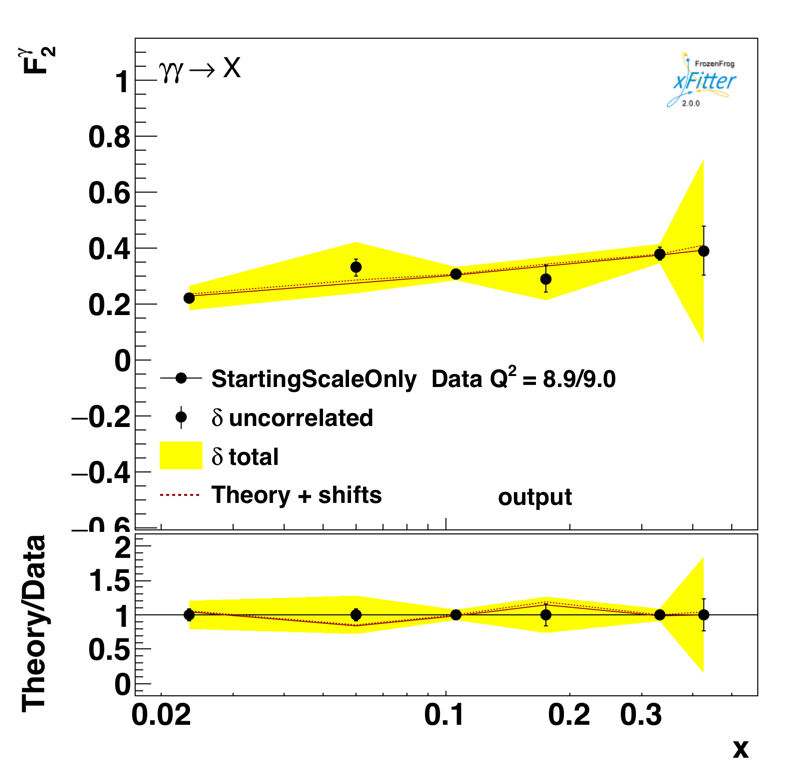
\includegraphics[width=0.4\linewidth]{/Users/schulte/F2_Analysis/10Prozent/Q2_9_0plot.png}
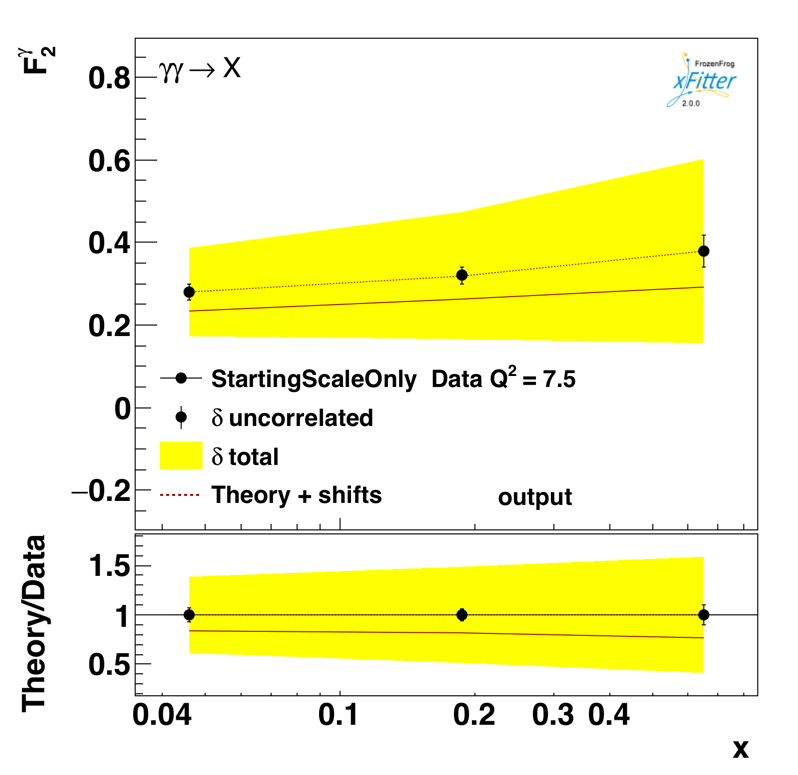
\includegraphics[width=0.4\linewidth]{/Users/schulte/F2_Analysis/10Prozent/Q2_7_5plot.png}\\

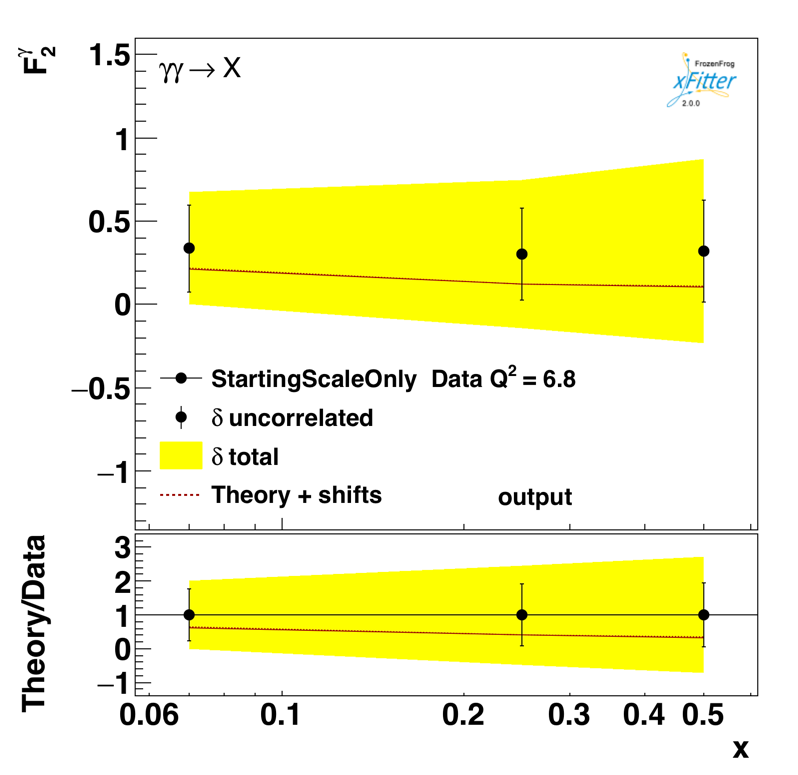
\includegraphics[width=0.4\linewidth]{/Users/schulte/F2_Analysis/10Prozent/Q2_6_8plot.png}
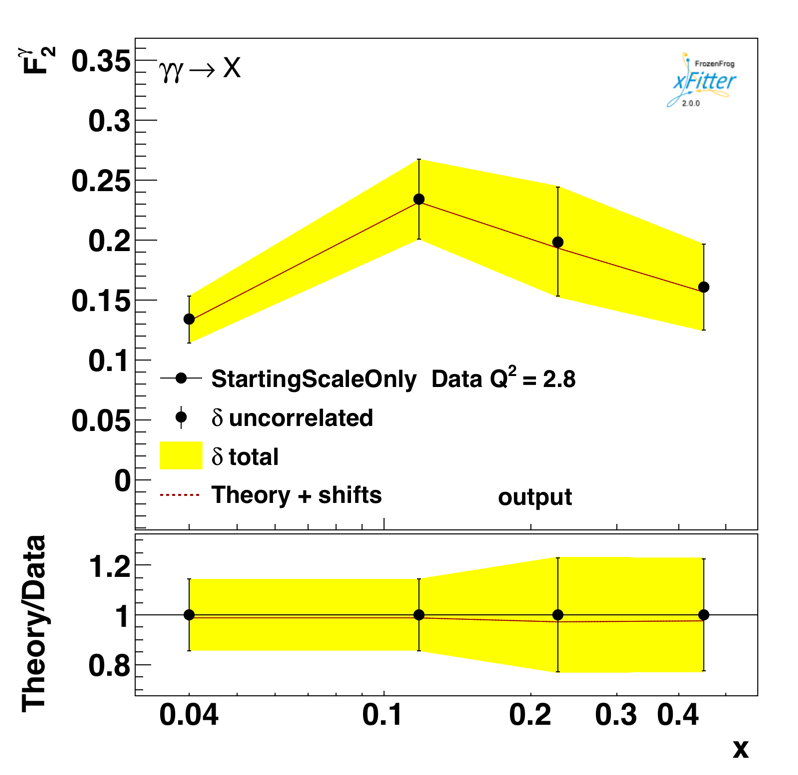
\includegraphics[width=0.4\linewidth]{/Users/schulte/F2_Analysis/10Prozent/Q2_2_8plot.png}\\

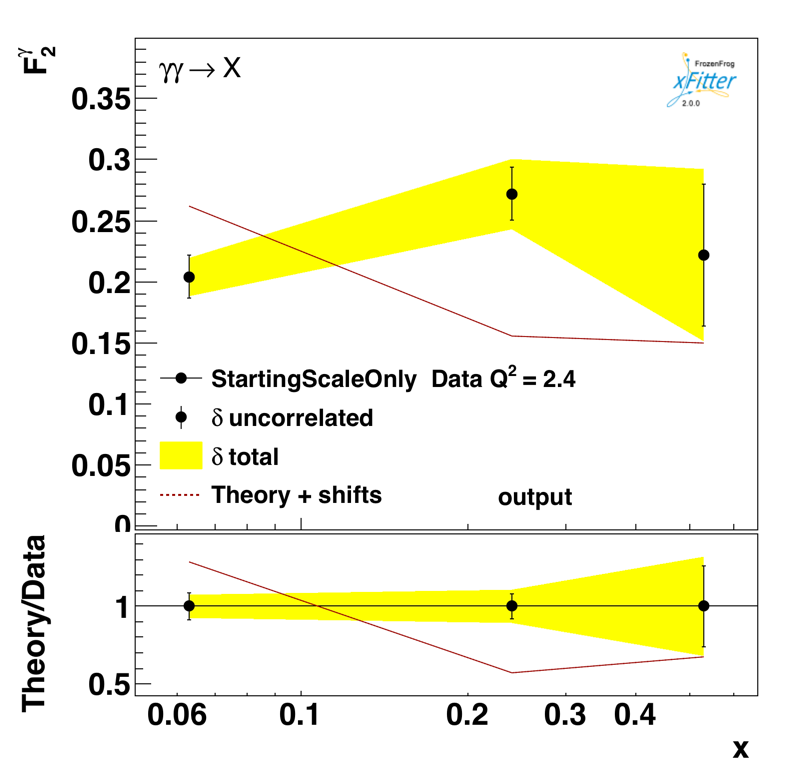
\includegraphics[width=0.4\linewidth]{/Users/schulte/F2_Analysis/10Prozent/Q2_2_4plot.png}
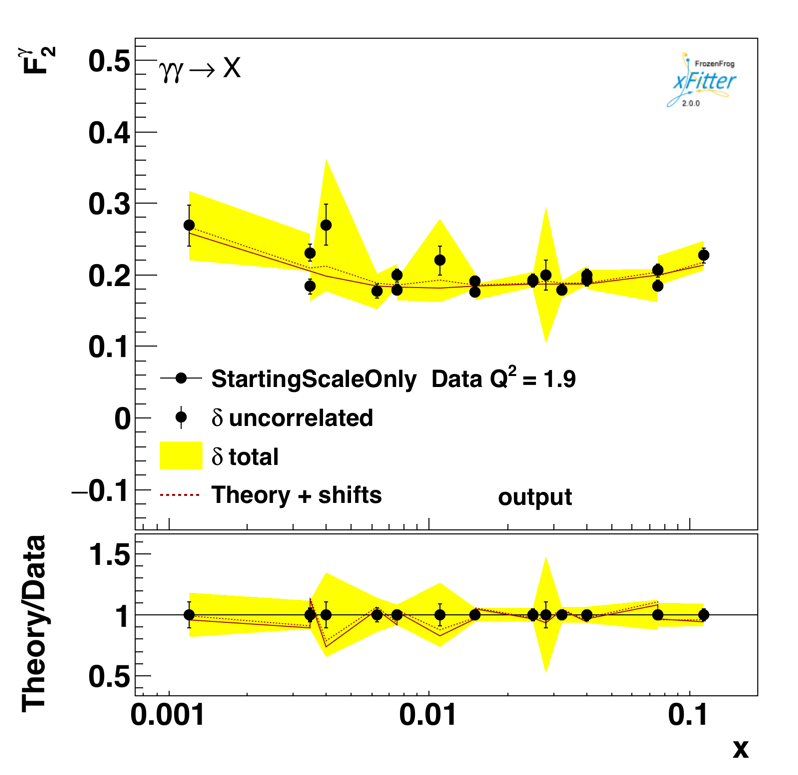
\includegraphics[width=0.4\linewidth]{/Users/schulte/F2_Analysis/10Prozent/Q2_1_9plot.png}
\\
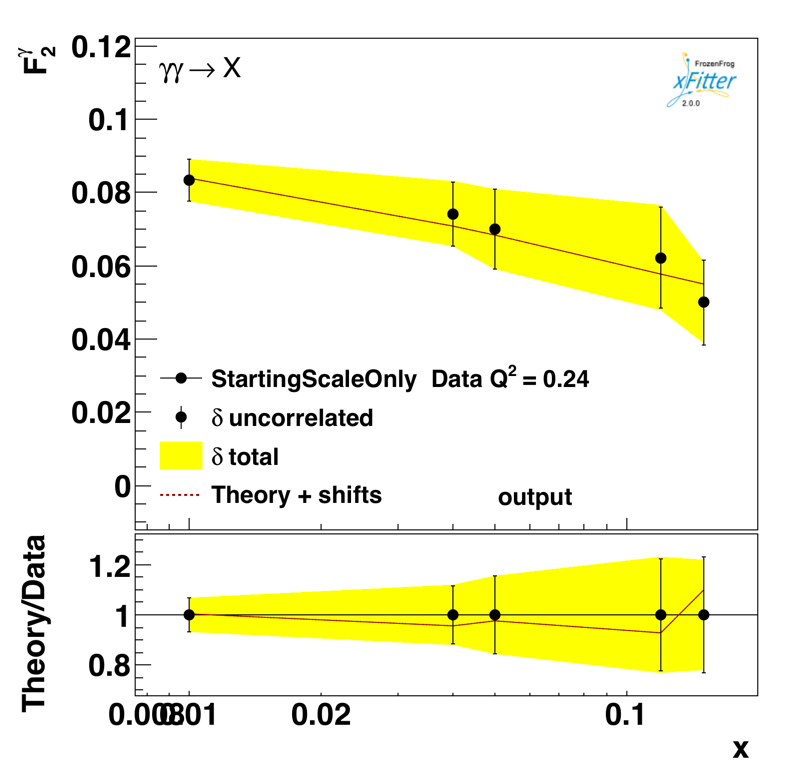
\includegraphics[width=0.4\linewidth]{/Users/schulte/F2_Analysis/10Prozent/Q2_0_24plot.png}
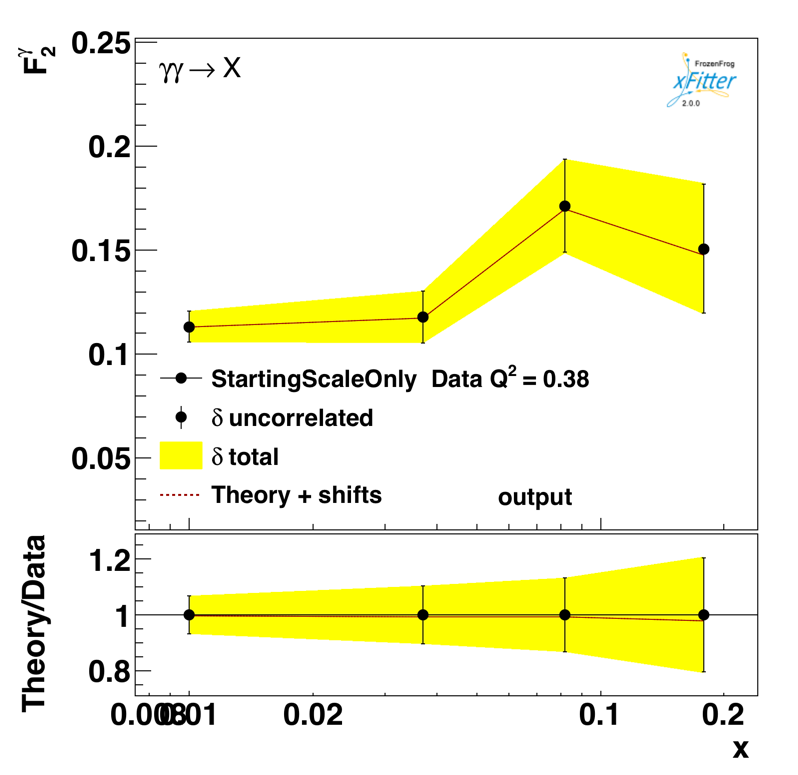
\includegraphics[width=0.4\linewidth]{/Users/schulte/F2_Analysis/10Prozent/Q2_0_38plot.png}\\

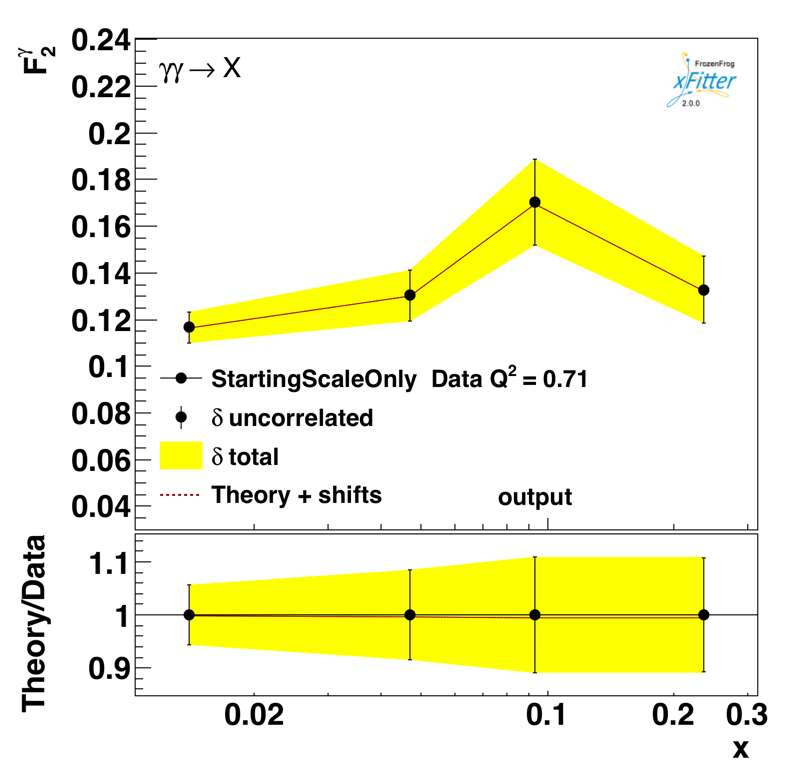
\includegraphics[width=0.4\linewidth]{/Users/schulte/F2_Analysis/10Prozent/Q2_0_71plot.png}
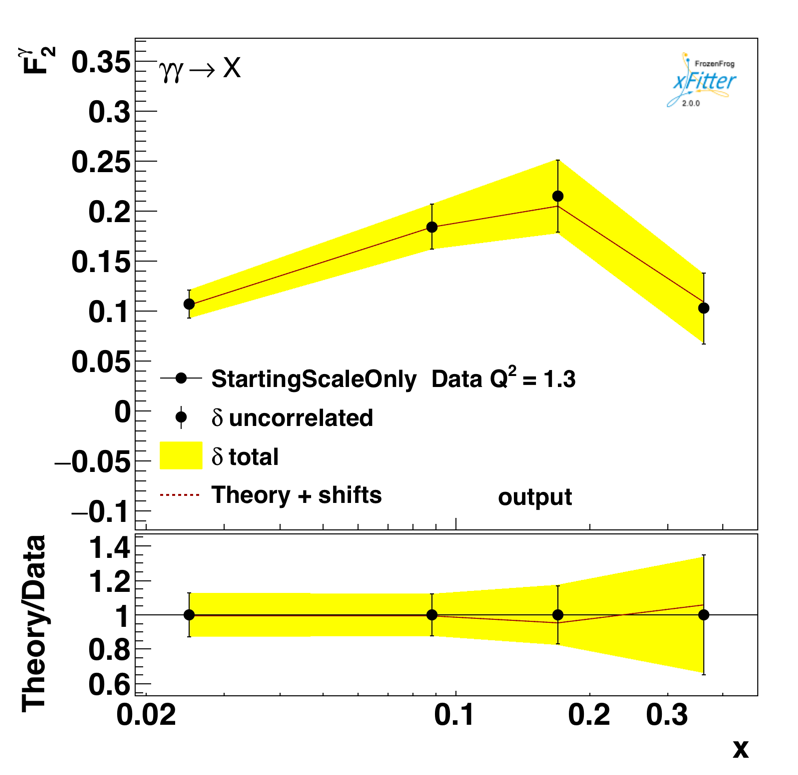
\includegraphics[width=0.4\linewidth]{/Users/schulte/F2_Analysis/10Prozent/Q2_1_3plot.png}
\\
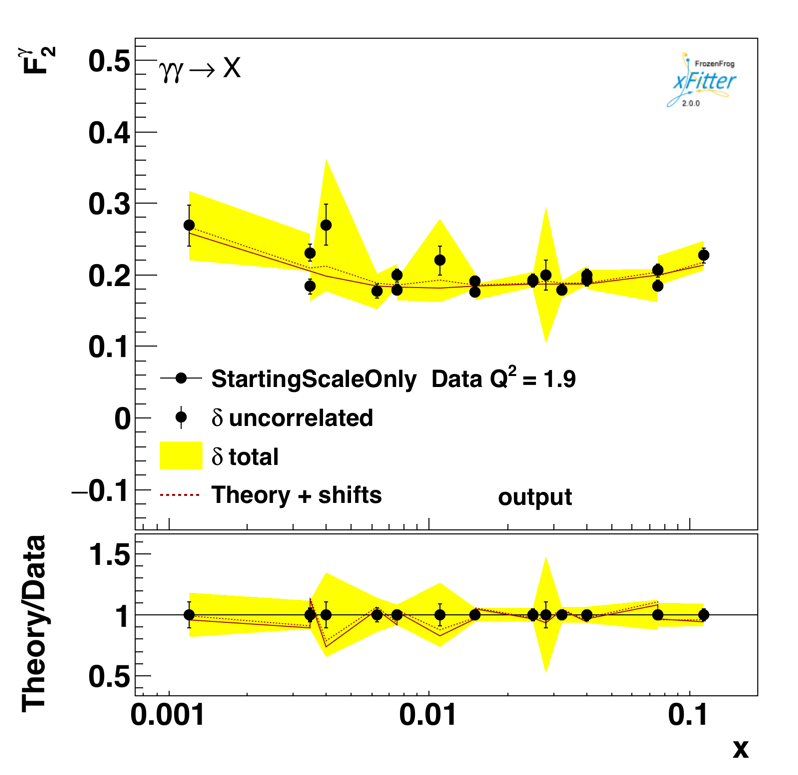
\includegraphics[width=0.4\linewidth]{/Users/schulte/F2_Analysis/10Prozent/Q2_1_9plot.png}
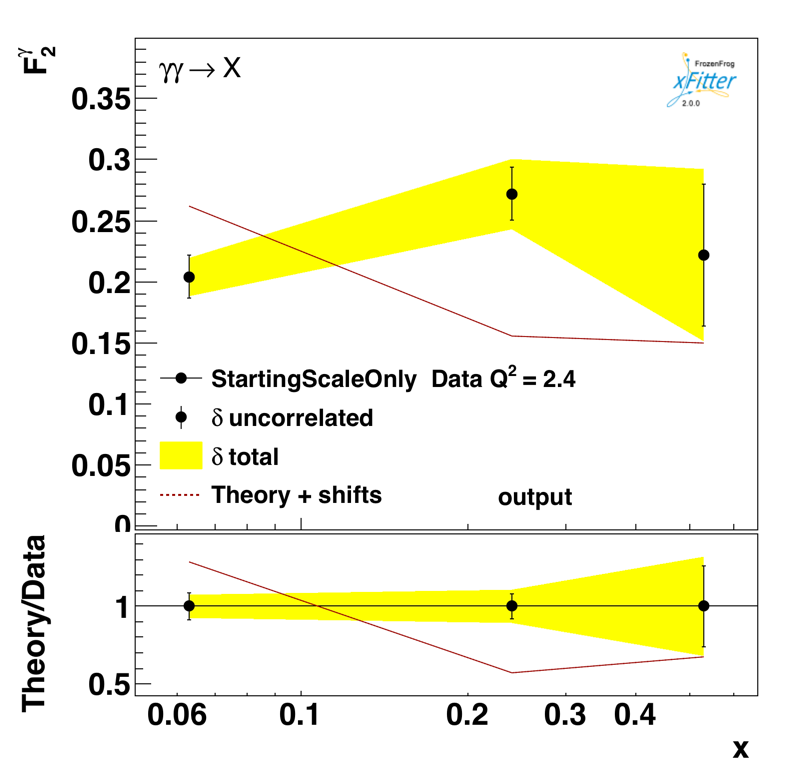
\includegraphics[width=0.4\linewidth]{/Users/schulte/F2_Analysis/10Prozent/Q2_2_4plot.png}
\\
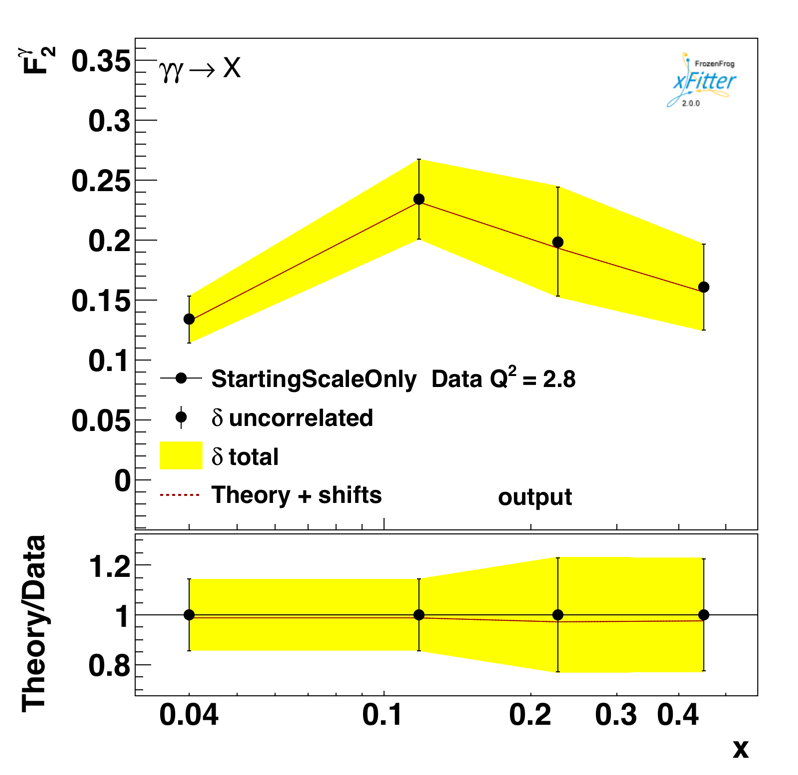
\includegraphics[width=0.4\linewidth]{/Users/schulte/F2_Analysis/10Prozent/Q2_2_8plot.png}
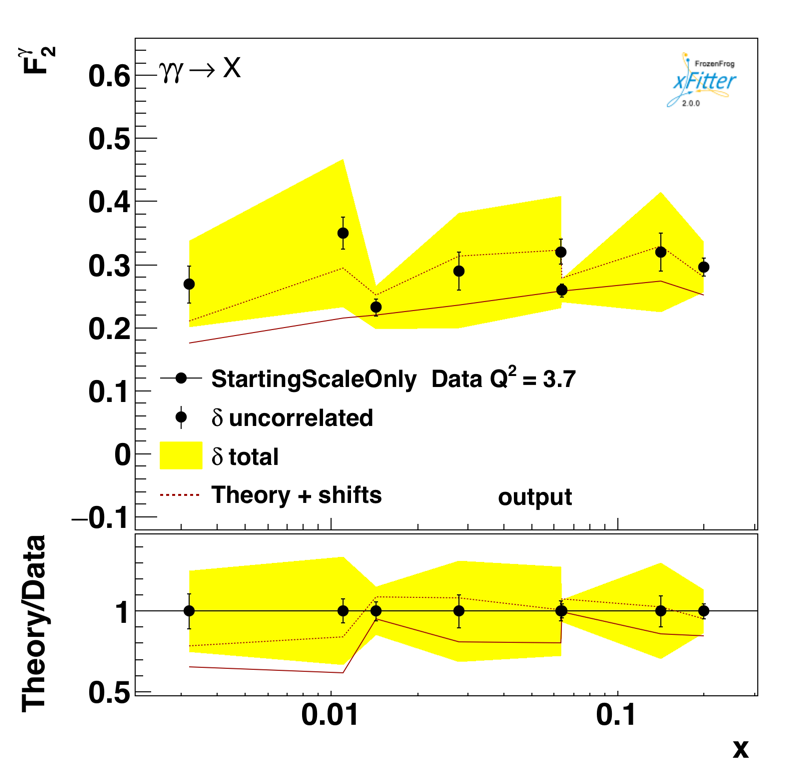
\includegraphics[width=0.4\linewidth]{/Users/schulte/F2_Analysis/10Prozent/Q2_3_7plot.png}
\\
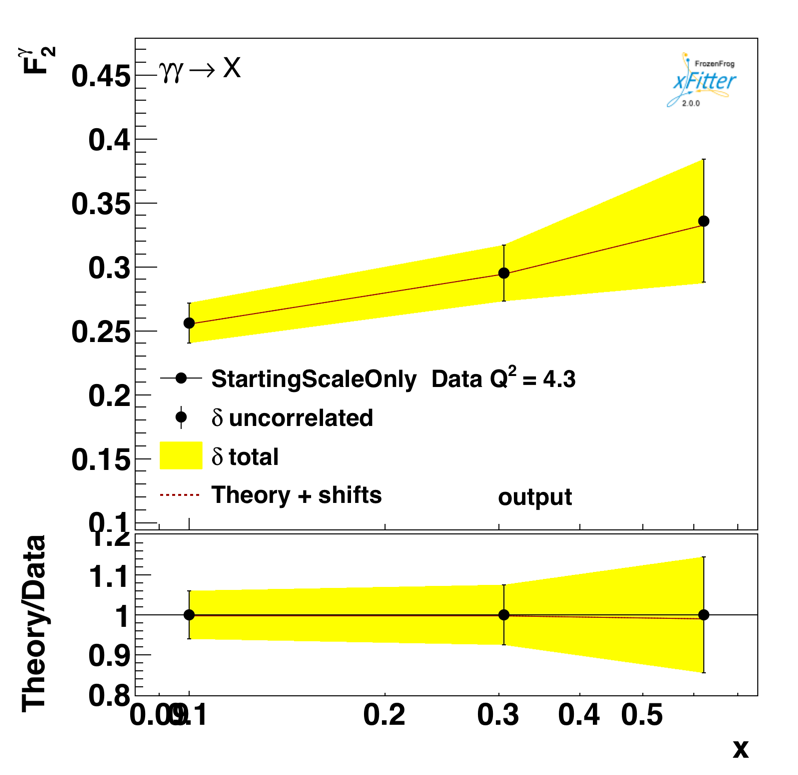
\includegraphics[width=0.4\linewidth]{/Users/schulte/F2_Analysis/10Prozent/Q2_4_3plot.png}
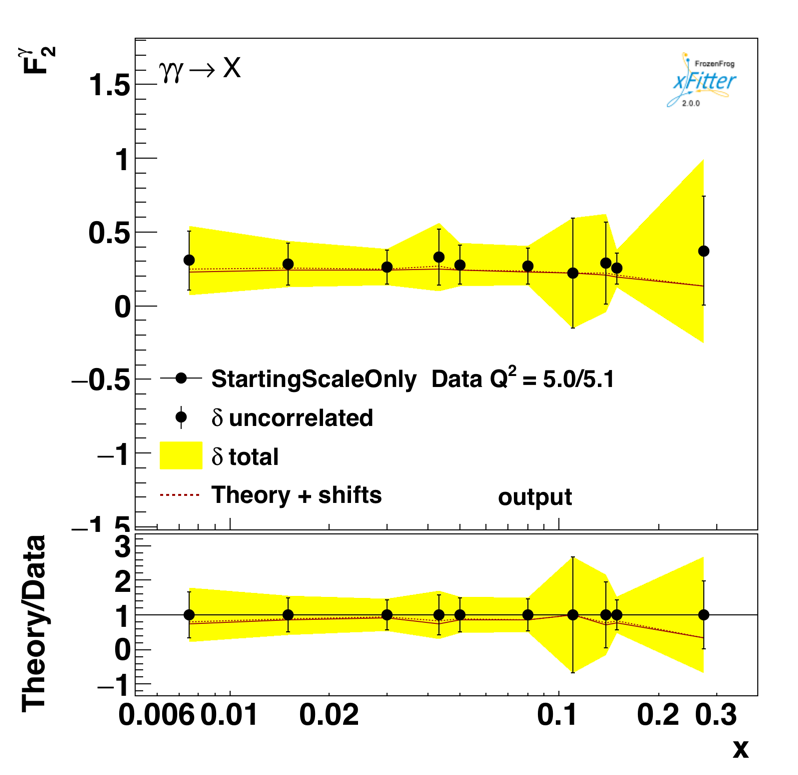
\includegraphics[width=0.4\linewidth]{/Users/schulte/F2_Analysis/10Prozent/Q2_5_0plot.png}\\

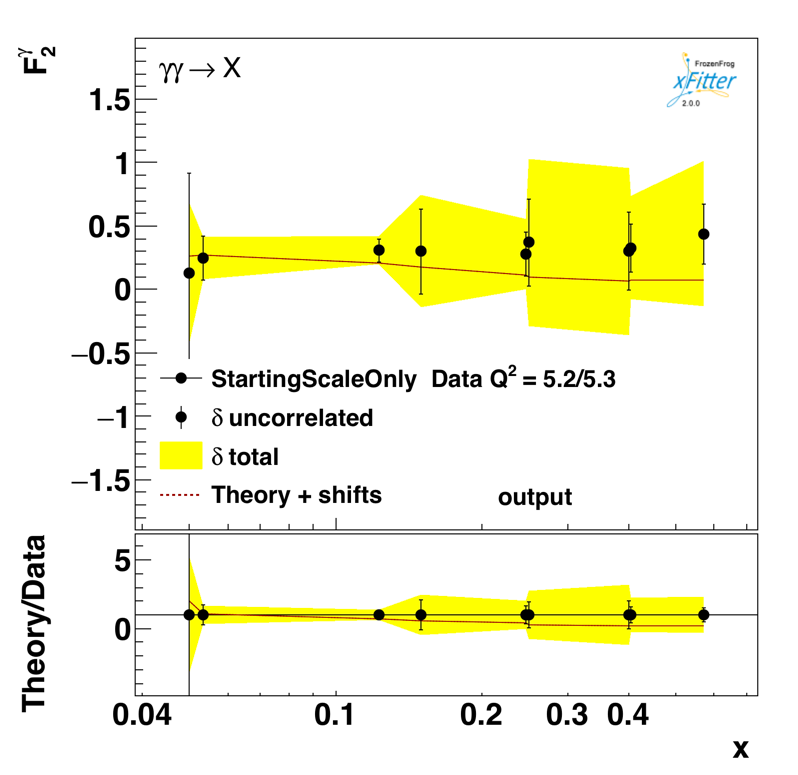
\includegraphics[width=0.4\linewidth]{/Users/schulte/F2_Analysis/10Prozent/Q2_5_3plot.png}
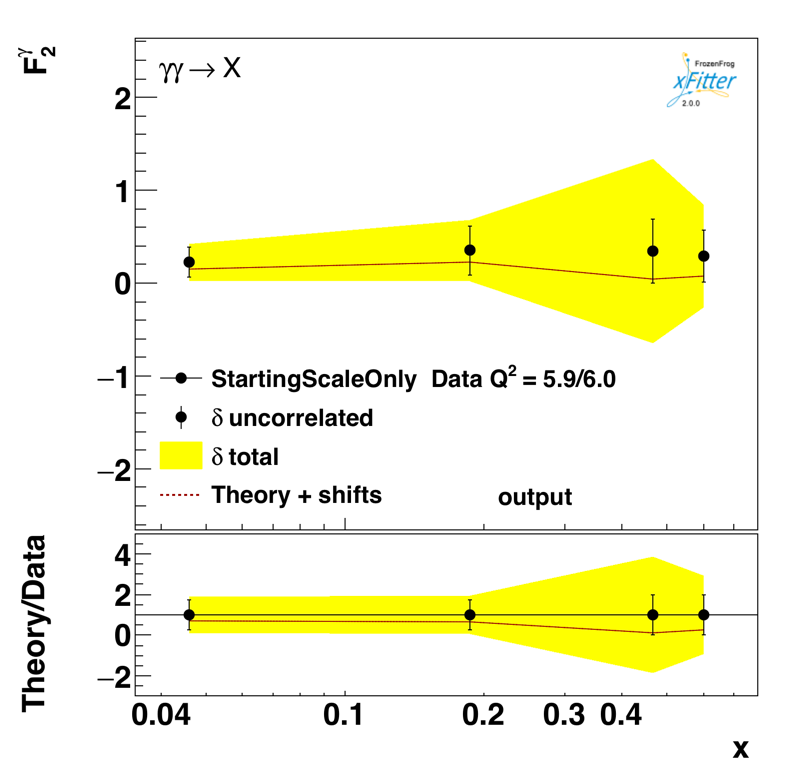
\includegraphics[width=0.4\linewidth]{/Users/schulte/F2_Analysis/10Prozent/Q2_5_9plot.png}\\

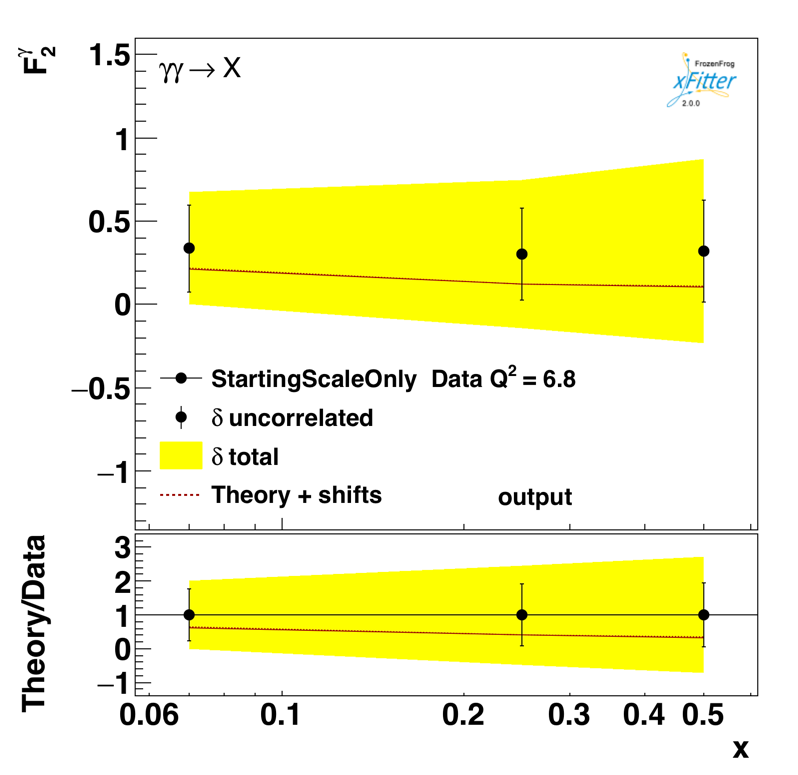
\includegraphics[width=0.4\linewidth]{/Users/schulte/F2_Analysis/10Prozent/Q2_6_8plot.png}
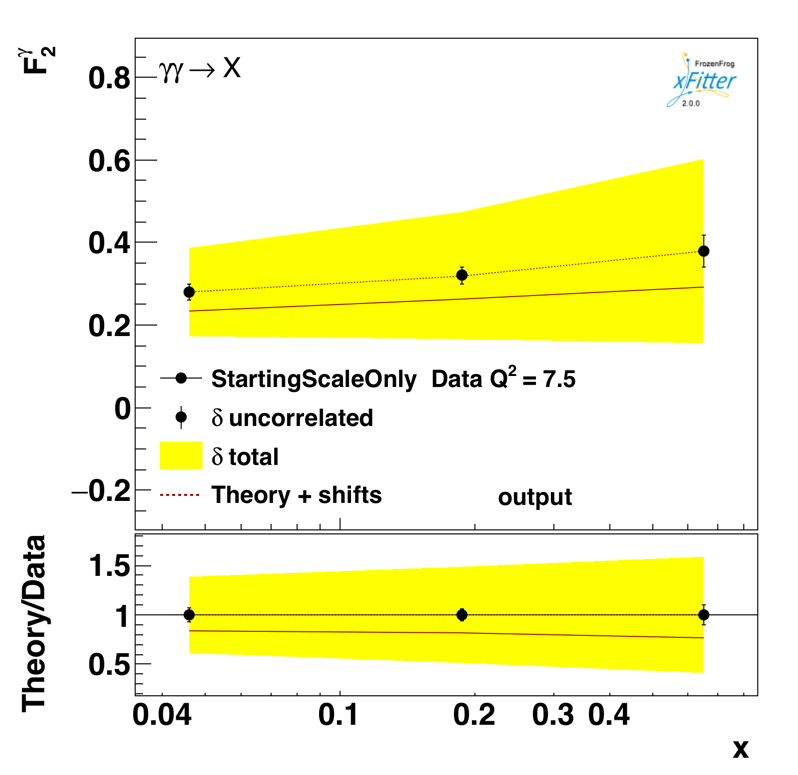
\includegraphics[width=0.4\linewidth]{/Users/schulte/F2_Analysis/10Prozent/Q2_7_5plot.png}\\

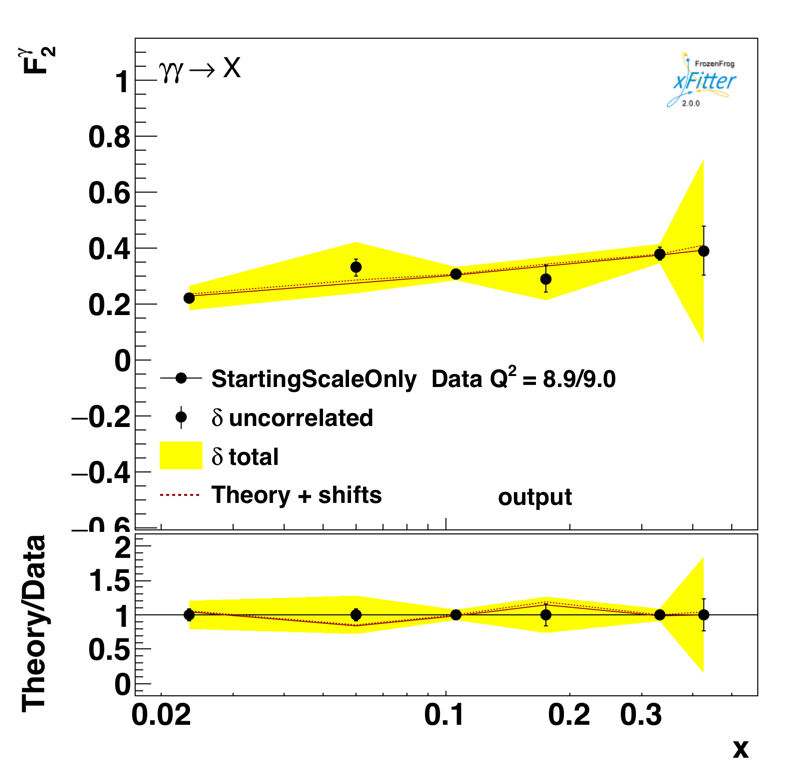
\includegraphics[width=0.4\linewidth]{/Users/schulte/F2_Analysis/10Prozent/Q2_9_0plot.png}
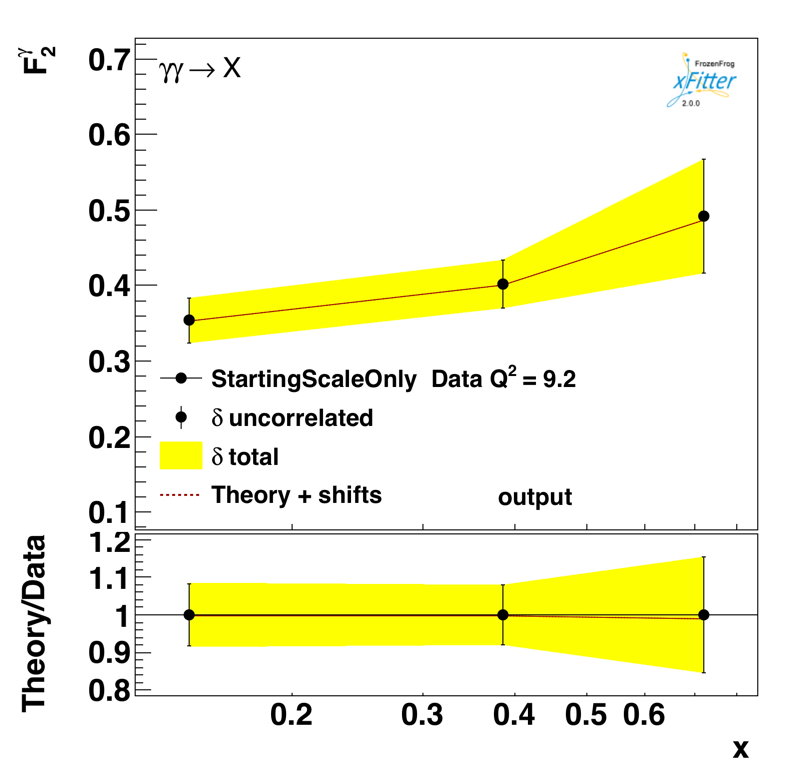
\includegraphics[width=0.4\linewidth]{/Users/schulte/F2_Analysis/10Prozent/Q2_9_2plot.png}\\

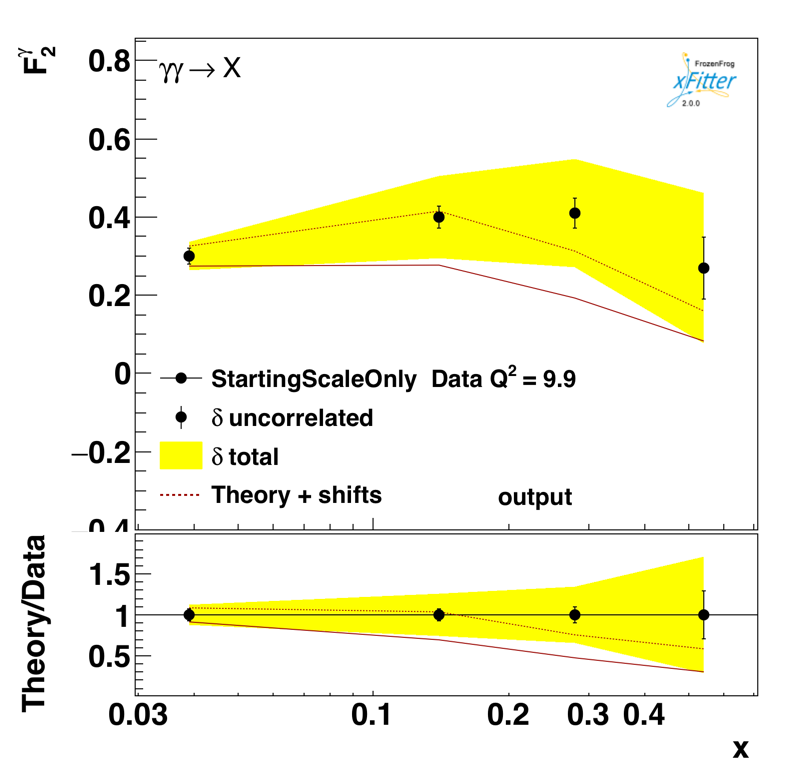
\includegraphics[width=0.4\linewidth]{/Users/schulte/F2_Analysis/10Prozent/Q2_9_9plot.png}
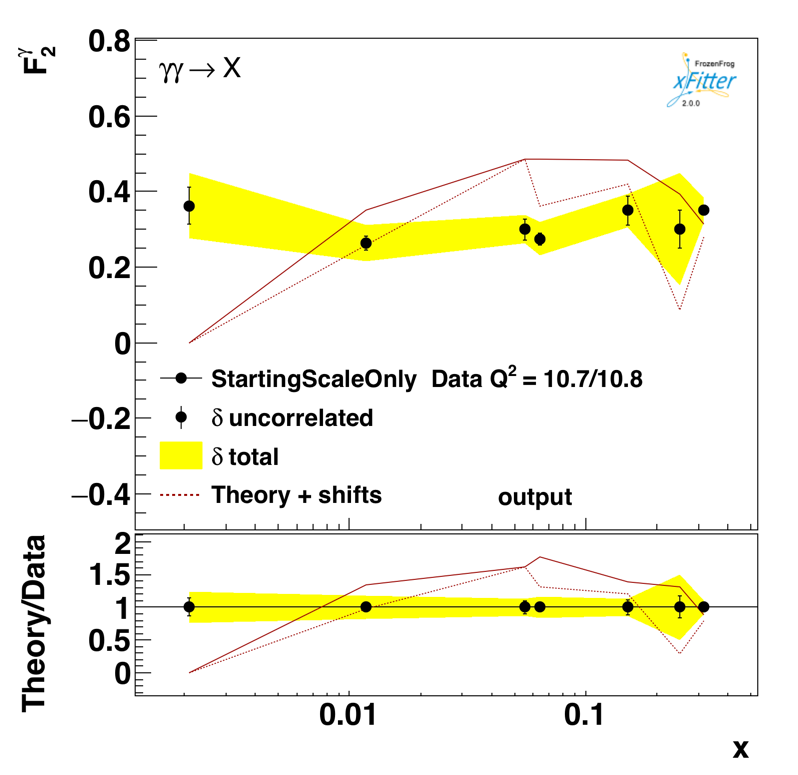
\includegraphics[width=0.4\linewidth]{/Users/schulte/F2_Analysis/10Prozent/Q2_10_8plot.png}\\

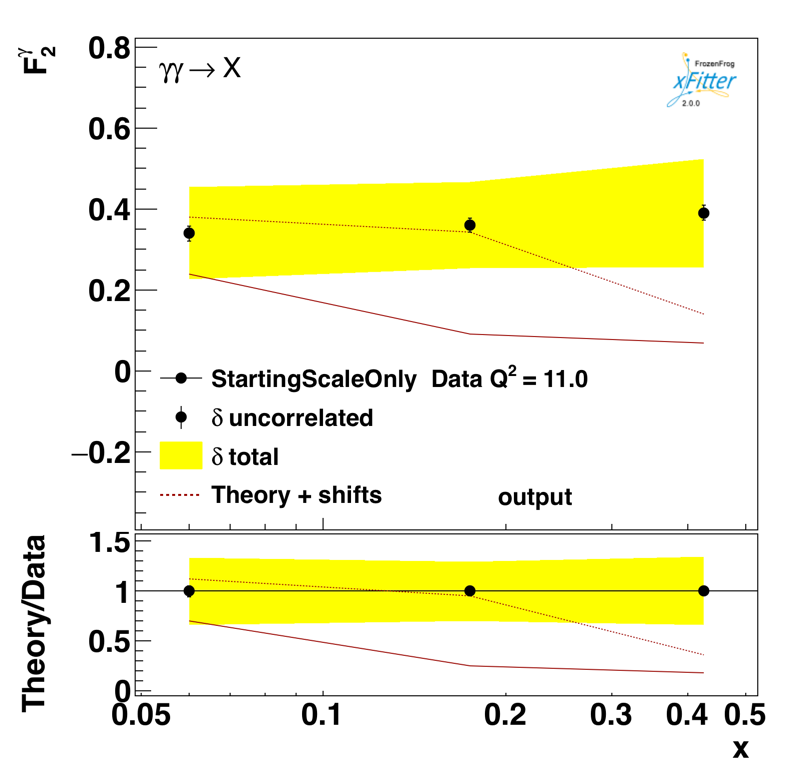
\includegraphics[width=0.4\linewidth]{/Users/schulte/F2_Analysis/10Prozent/Q2_11_0plot.png}
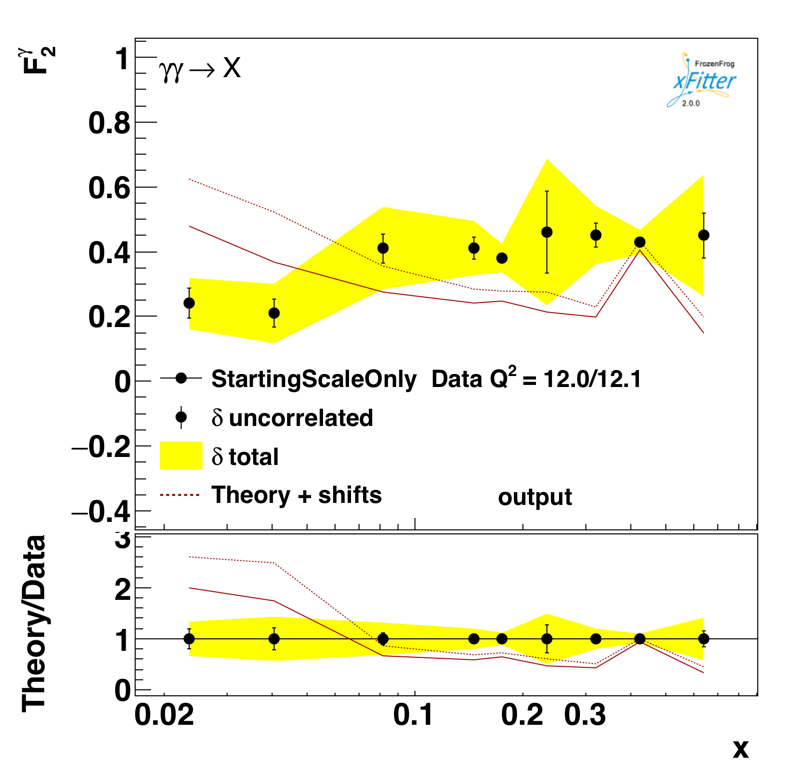
\includegraphics[width=0.4\linewidth]{/Users/schulte/F2_Analysis/10Prozent/Q2_12_0plot.png}\\
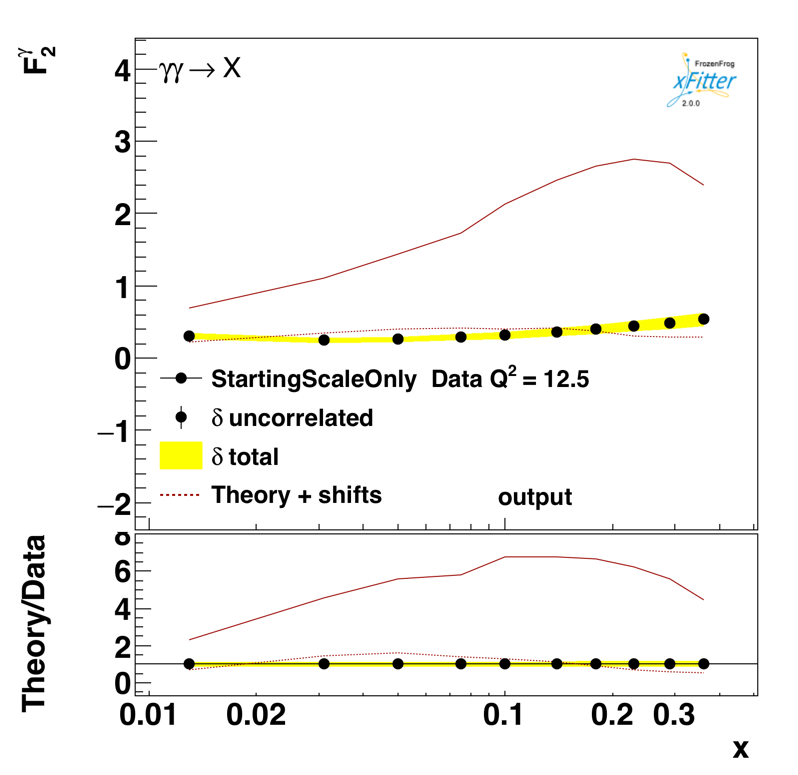
\includegraphics[width=0.4\linewidth]{/Users/schulte/F2_Analysis/10Prozent/Q2_12_5plot.png}
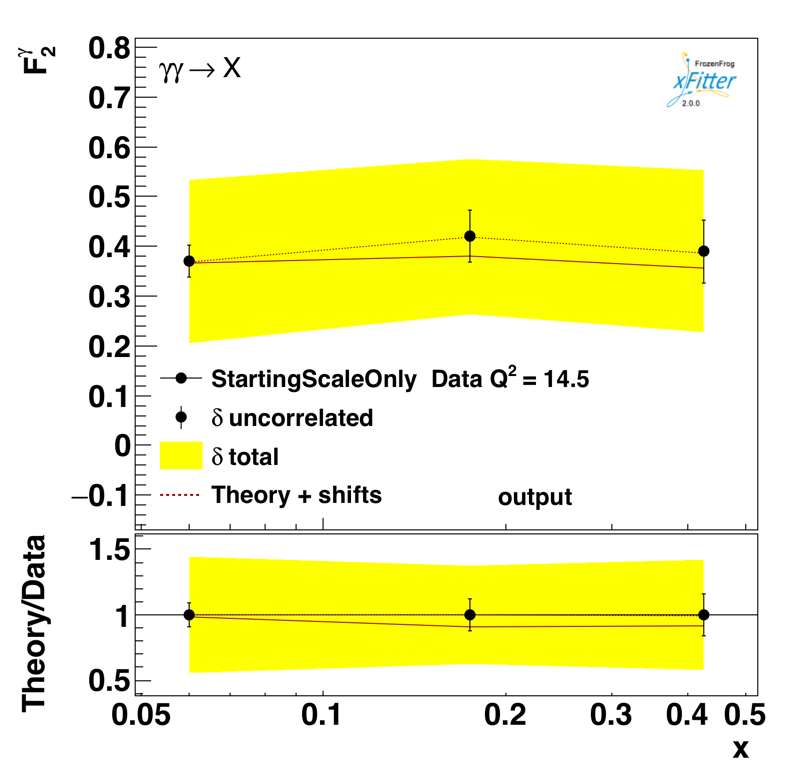
\includegraphics[width=0.4\linewidth]{/Users/schulte/F2_Analysis/10Prozent/Q2_14_5plot.png}\\

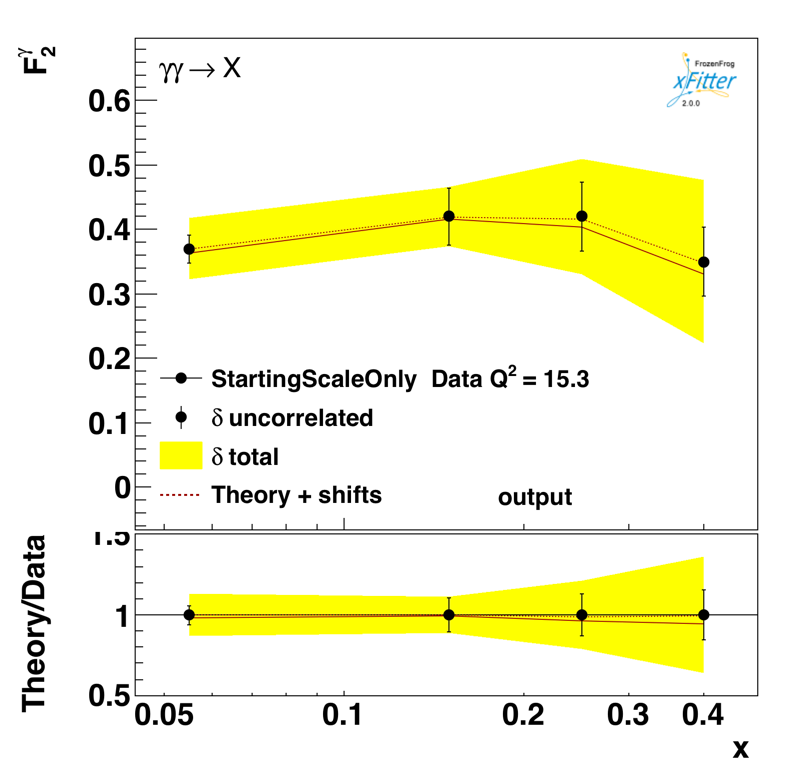
\includegraphics[width=0.4\linewidth]{/Users/schulte/F2_Analysis/10Prozent/Q2_15_3plot.png}
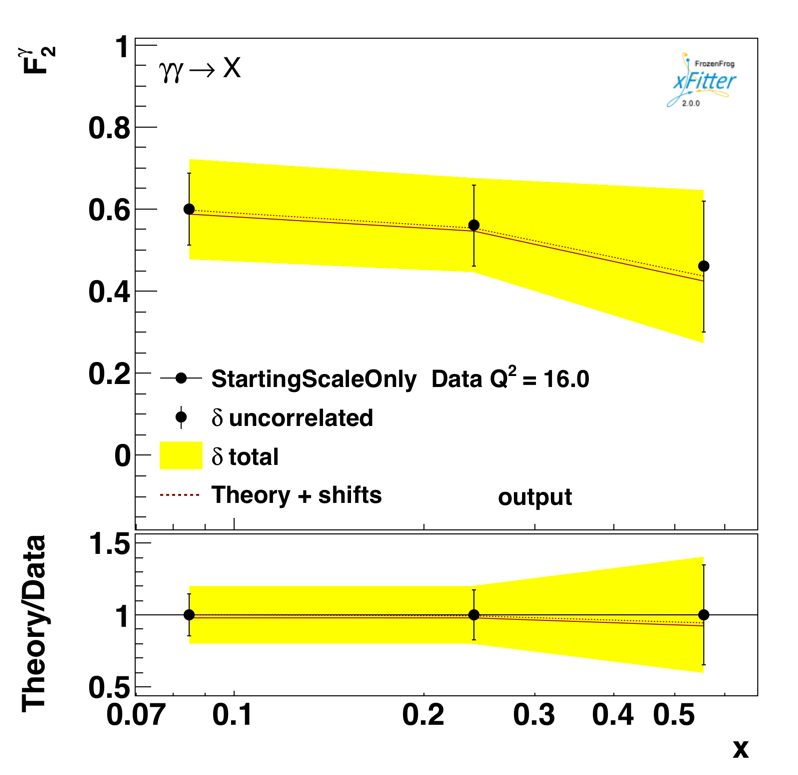
\includegraphics[width=0.4\linewidth]{/Users/schulte/F2_Analysis/10Prozent/Q2_16_0plot.png}\\

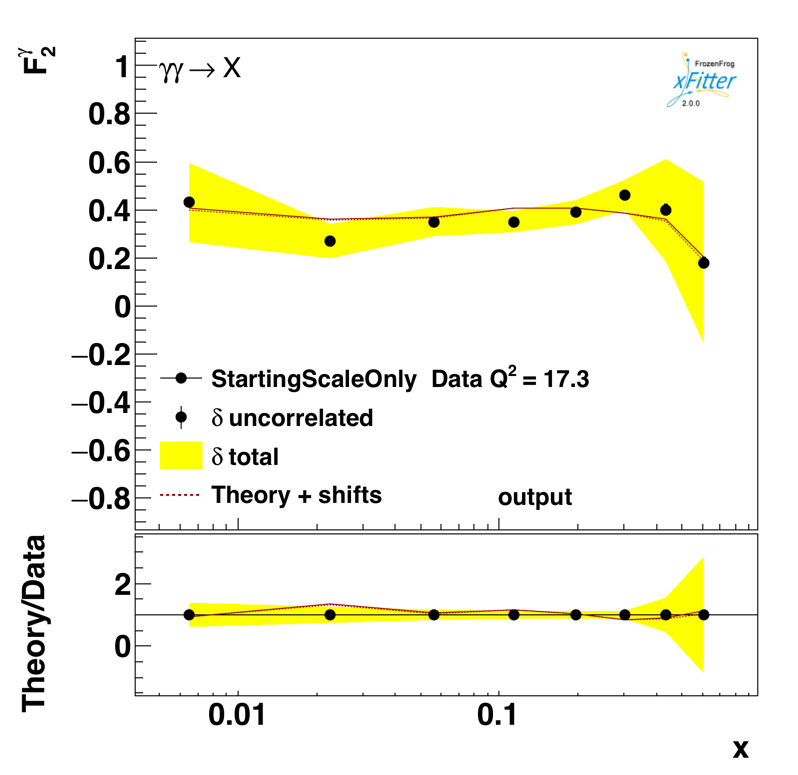
\includegraphics[width=0.4\linewidth]{/Users/schulte/F2_Analysis/10Prozent/Q2_17_3plot.png}
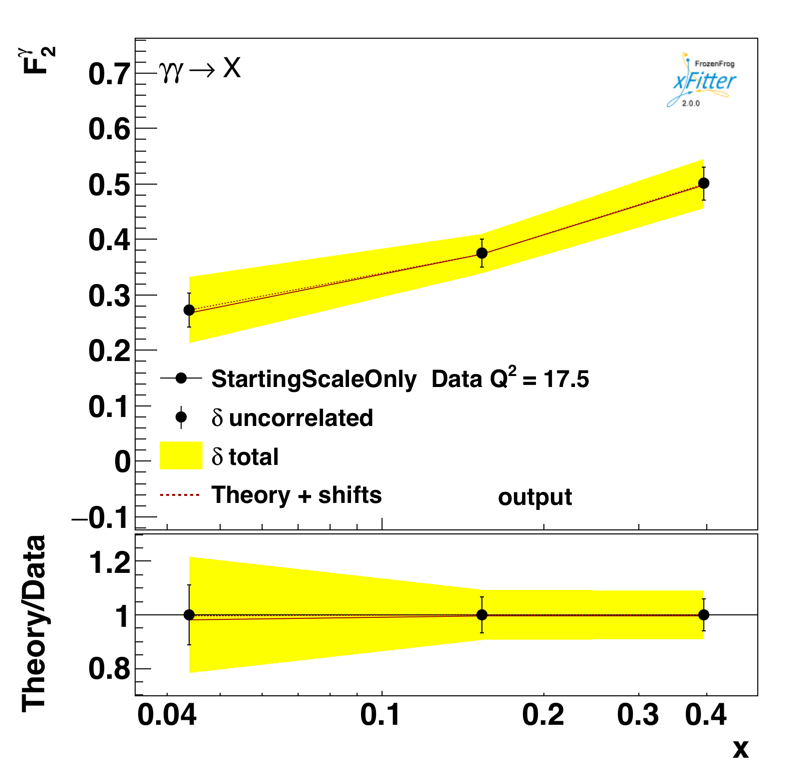
\includegraphics[width=0.4\linewidth]{/Users/schulte/F2_Analysis/10Prozent/Q2_17_5plot.png}\\

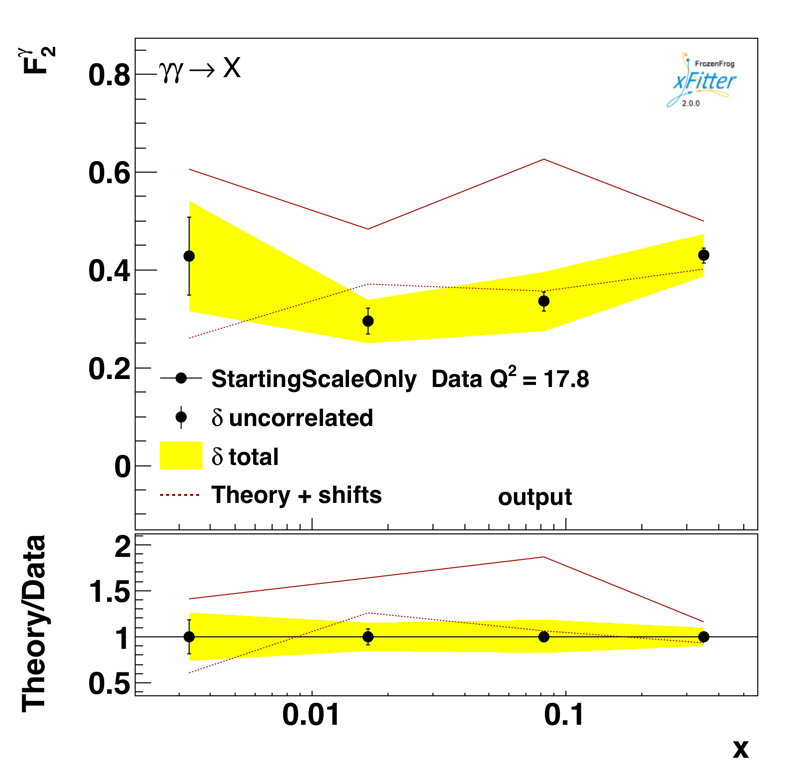
\includegraphics[width=0.4\linewidth]{/Users/schulte/F2_Analysis/10Prozent/Q2_17_8plot.png}
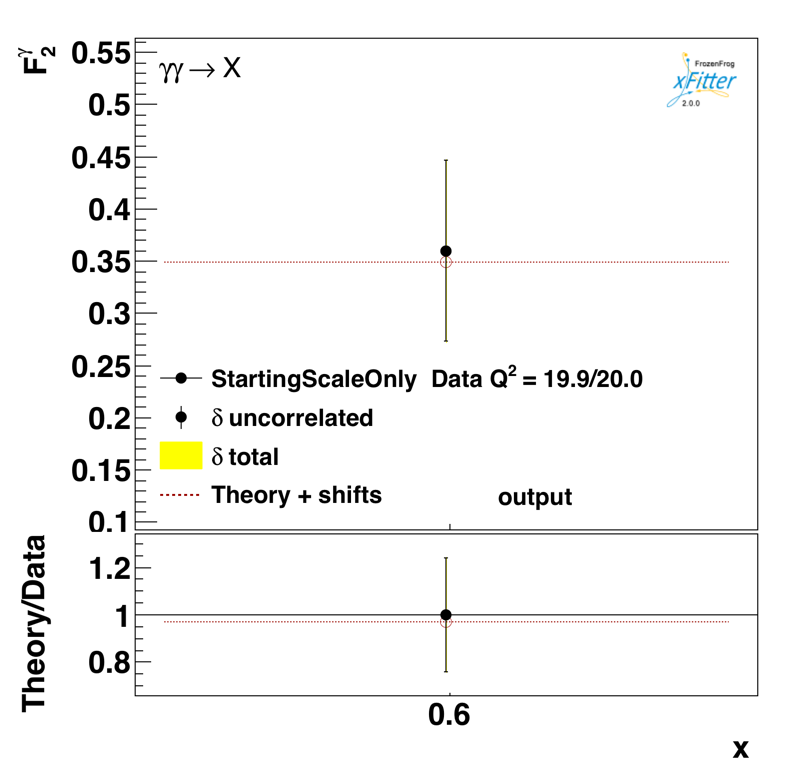
\includegraphics[width=0.4\linewidth]{/Users/schulte/F2_Analysis/10Prozent/Q2_20_0plot.png}\\

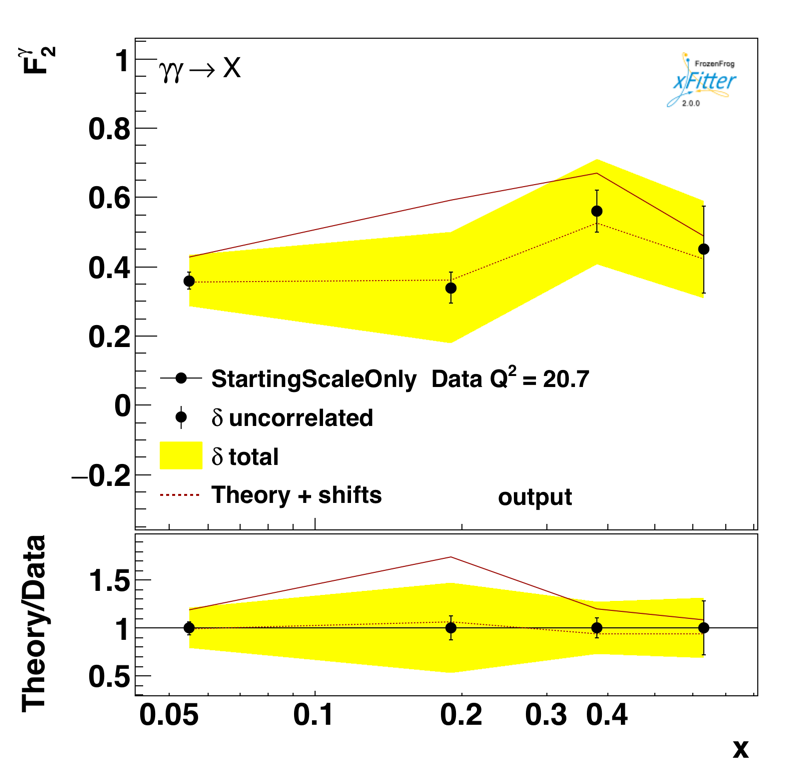
\includegraphics[width=0.4\linewidth]{/Users/schulte/F2_Analysis/10Prozent/Q2_20_7plot.png}
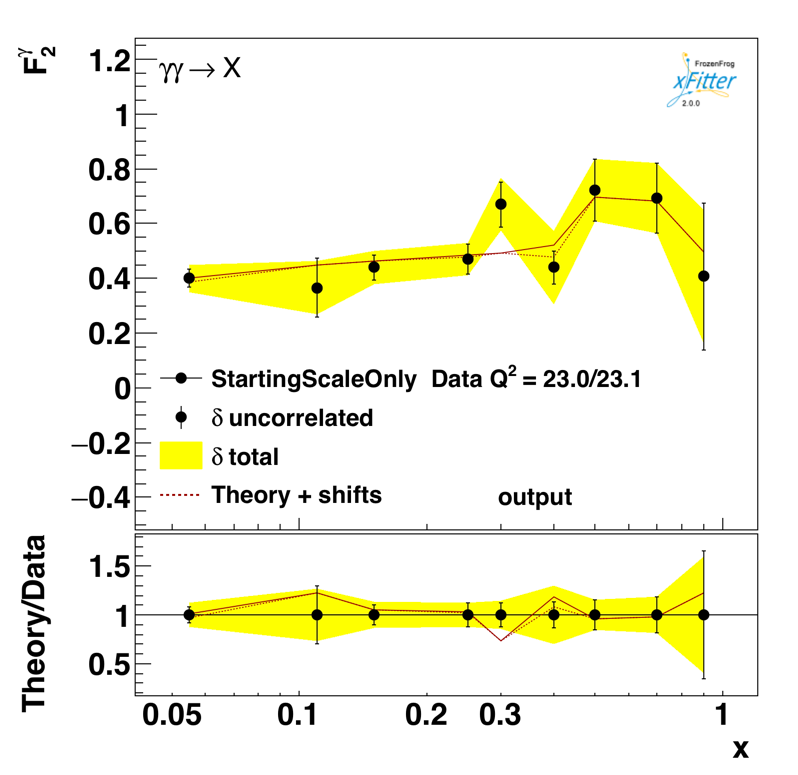
\includegraphics[width=0.4\linewidth]{/Users/schulte/F2_Analysis/10Prozent/Q2_23_0plot.png}\\

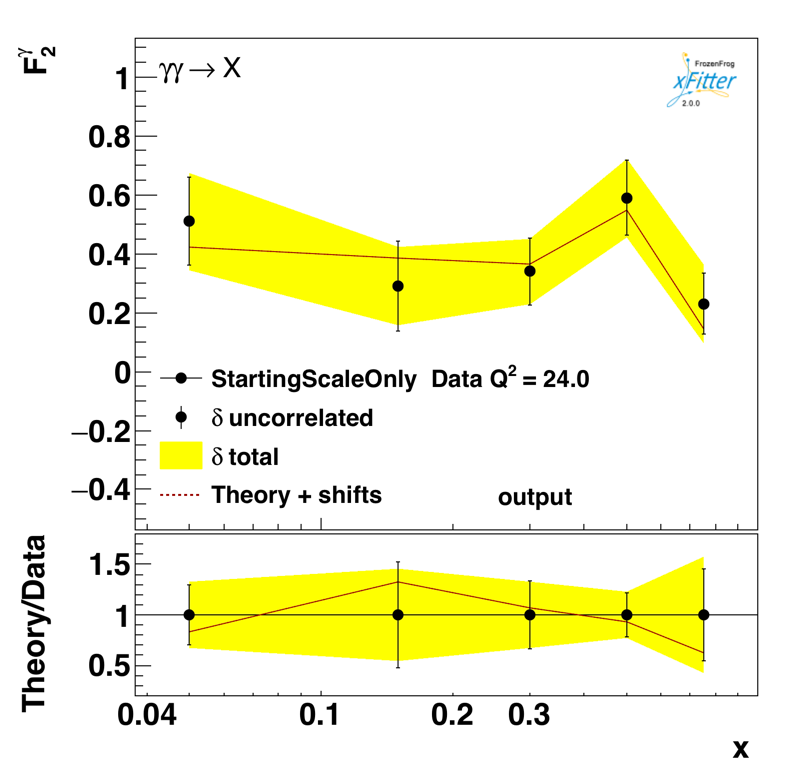
\includegraphics[width=0.4\linewidth]{/Users/schulte/F2_Analysis/10Prozent/Q2_24_0plot.png}
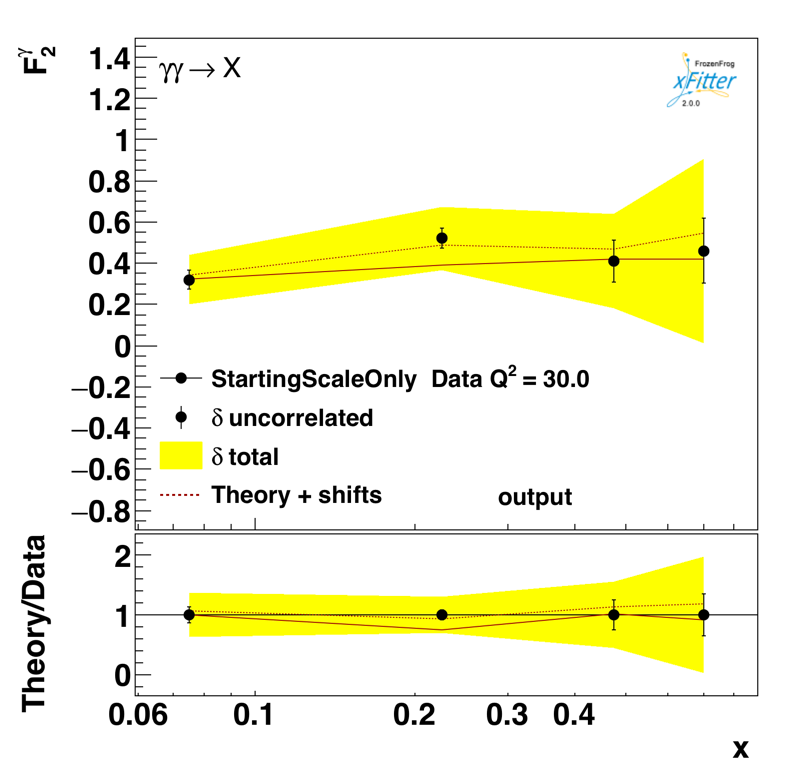
\includegraphics[width=0.4\linewidth]{/Users/schulte/F2_Analysis/10Prozent/Q2_30_0plot.png}\\

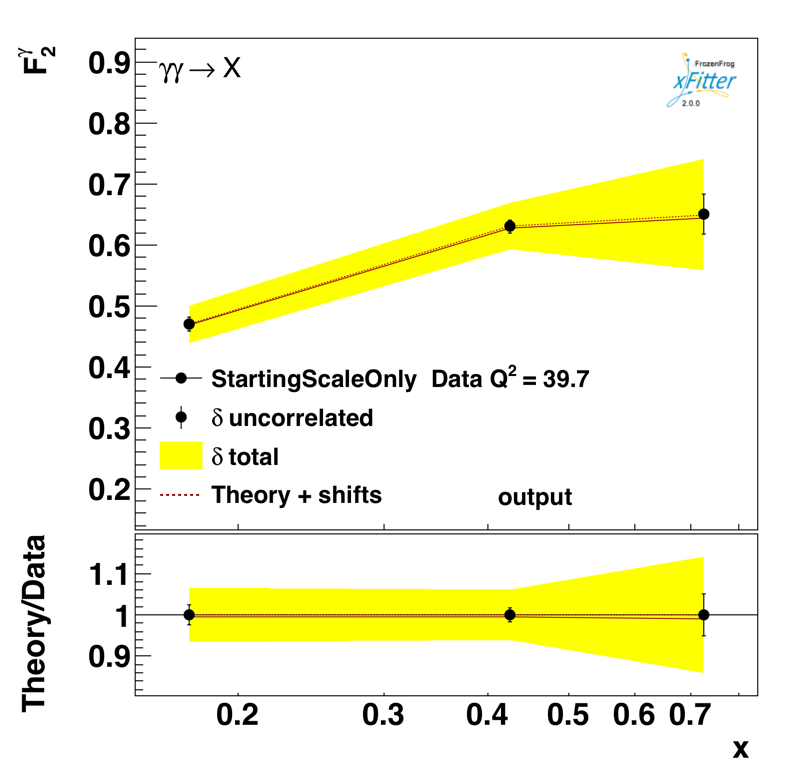
\includegraphics[width=0.4\linewidth]{/Users/schulte/F2_Analysis/10Prozent/Q2_39_7plot.png}
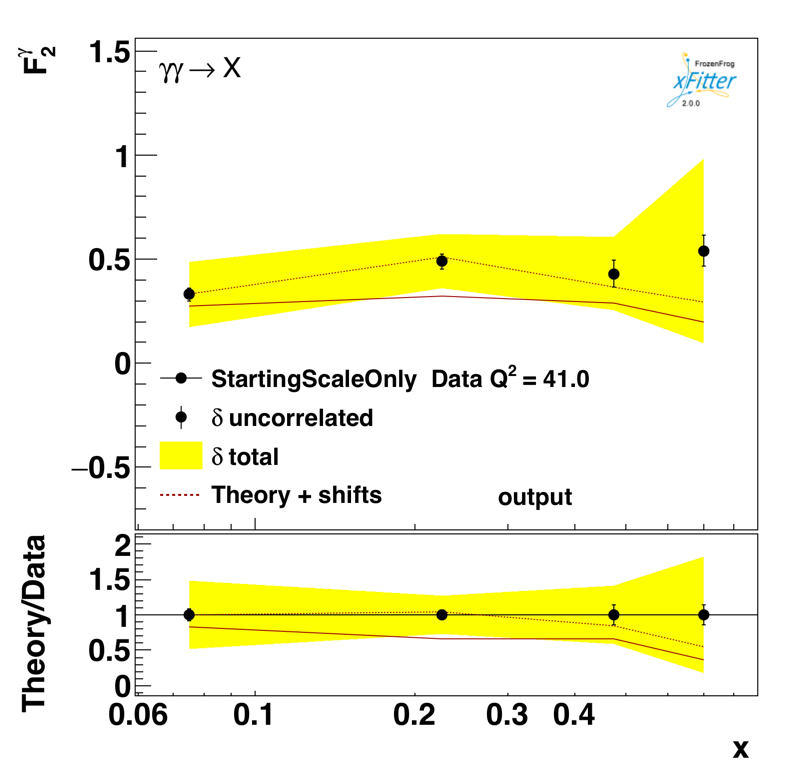
\includegraphics[width=0.4\linewidth]{/Users/schulte/F2_Analysis/10Prozent/Q2_41_0plot.png}\\

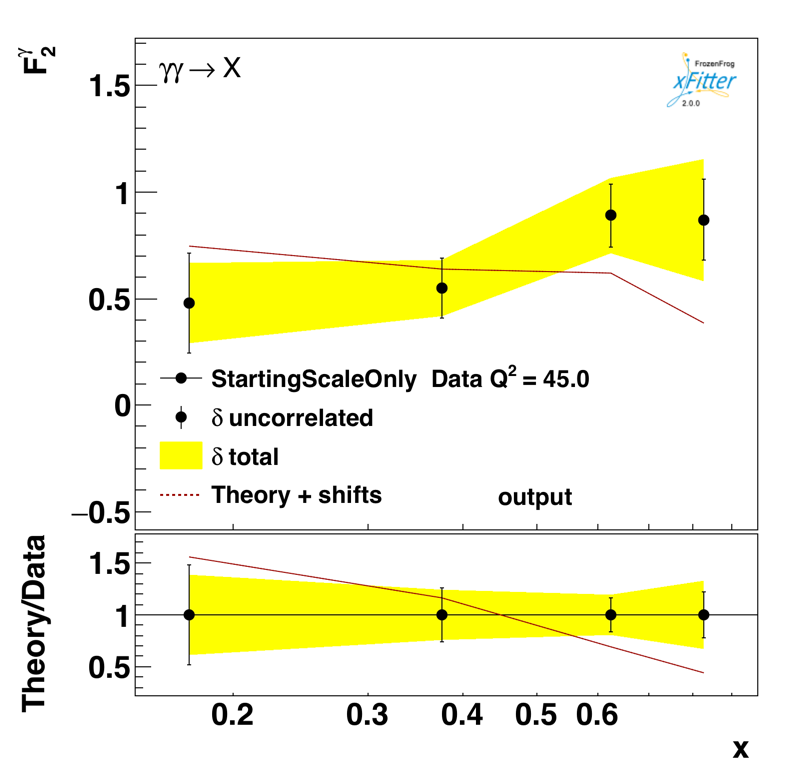
\includegraphics[width=0.4\linewidth]{/Users/schulte/F2_Analysis/10Prozent/Q2_45_0plot.png}
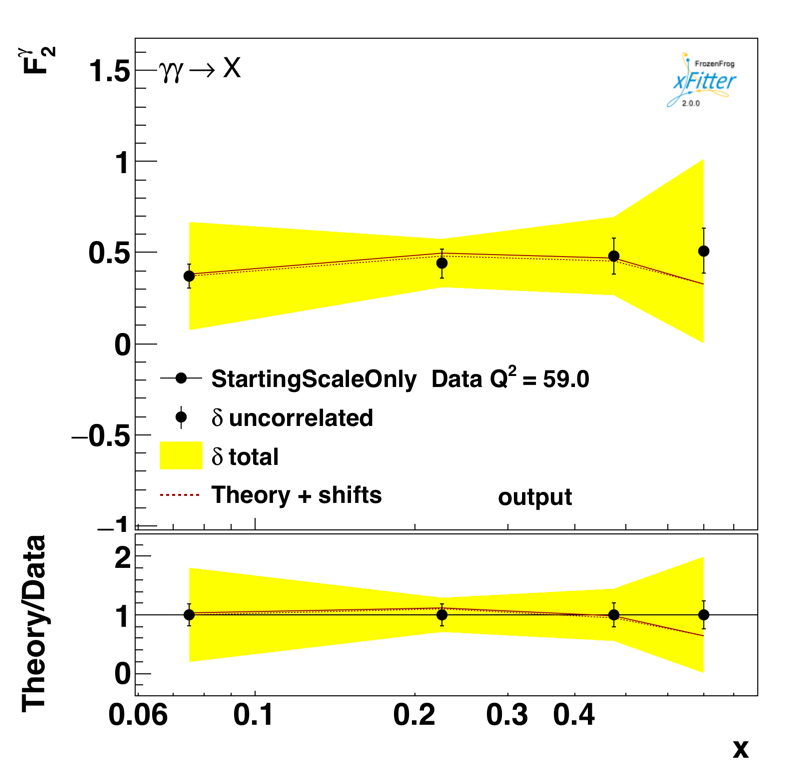
\includegraphics[width=0.4\linewidth]{/Users/schulte/F2_Analysis/10Prozent/Q2_59_0plot.png}\\

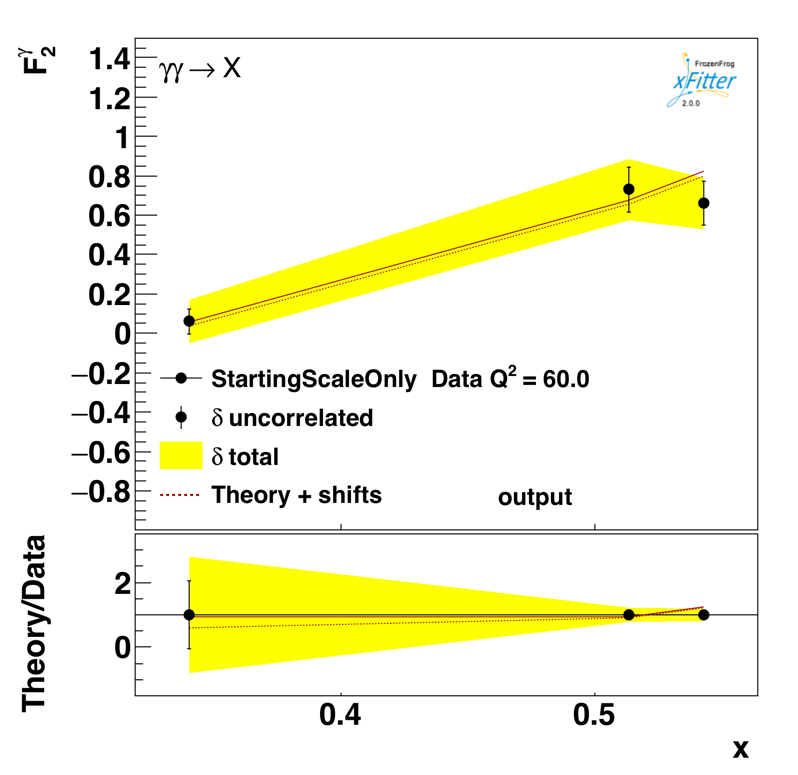
\includegraphics[width=0.4\linewidth]{/Users/schulte/F2_Analysis/10Prozent/Q2_60_0plot.png}
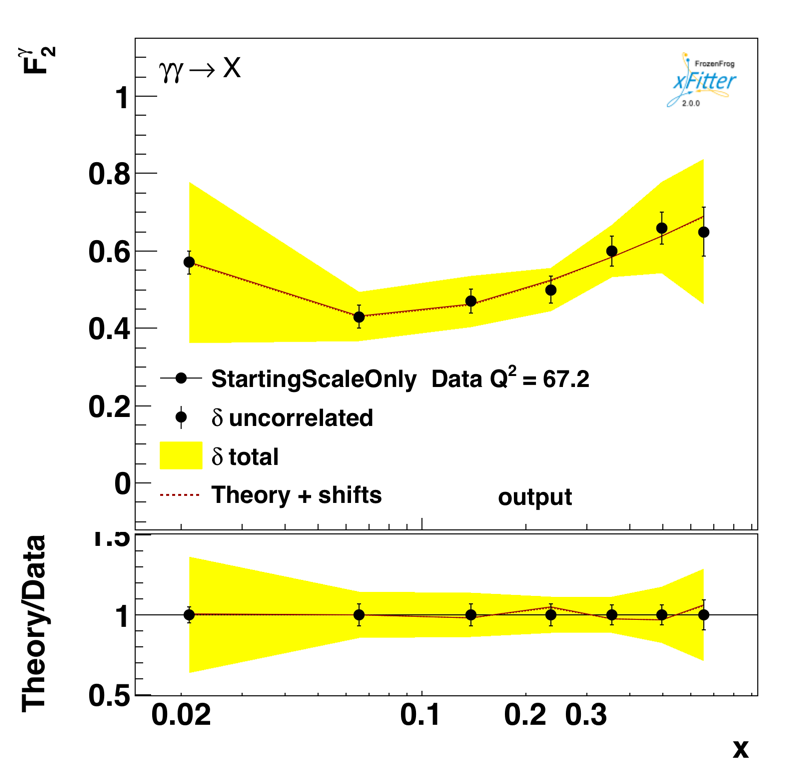
\includegraphics[width=0.4\linewidth]{/Users/schulte/F2_Analysis/10Prozent/Q2_67_2plot.png}\\

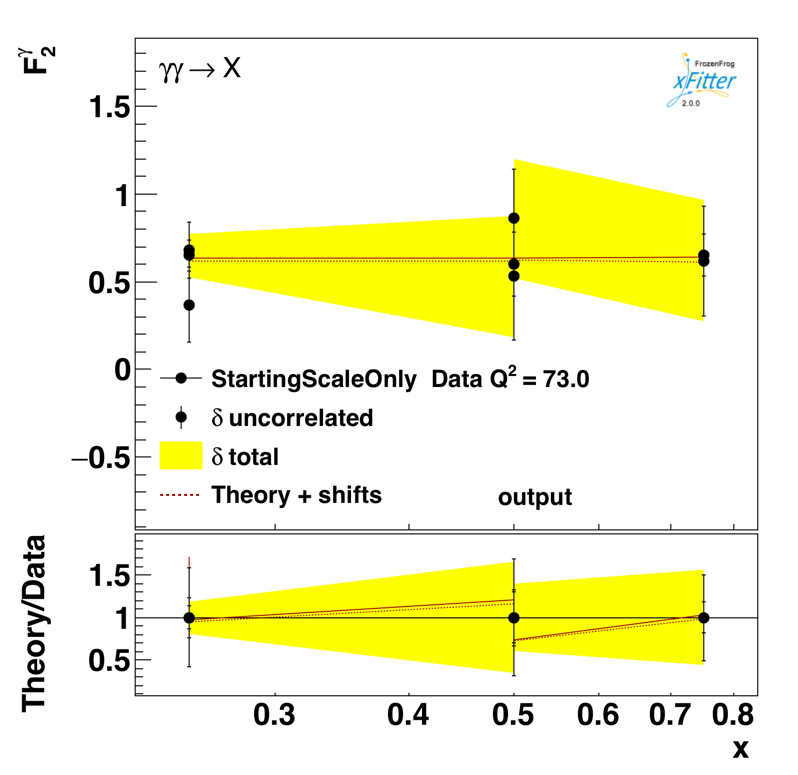
\includegraphics[width=0.4\linewidth]{/Users/schulte/F2_Analysis/10Prozent/Q2_73_0plot.png}
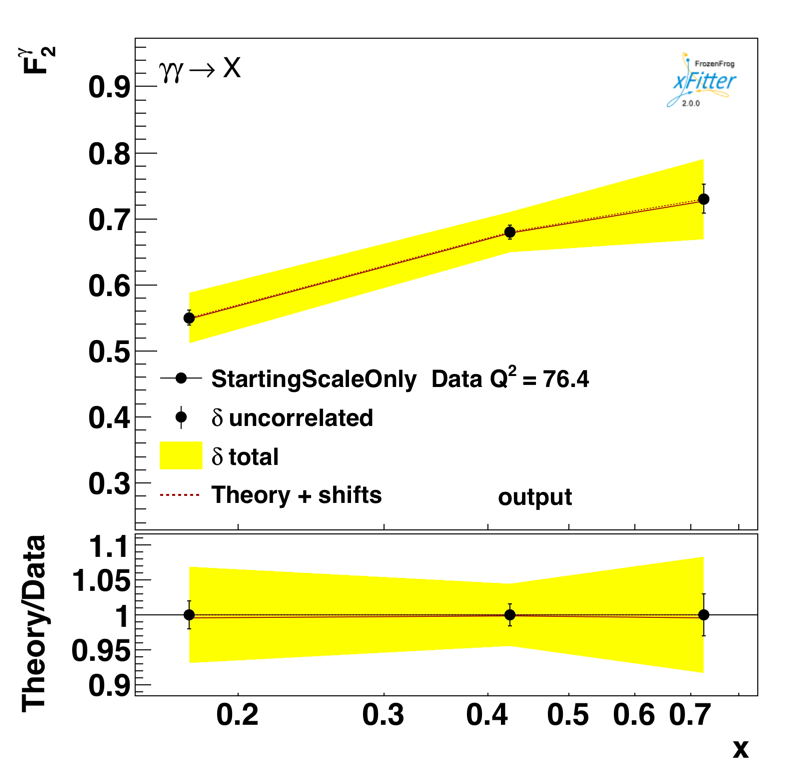
\includegraphics[width=0.4\linewidth]{/Users/schulte/F2_Analysis/10Prozent/Q2_76_4plot.png}\\

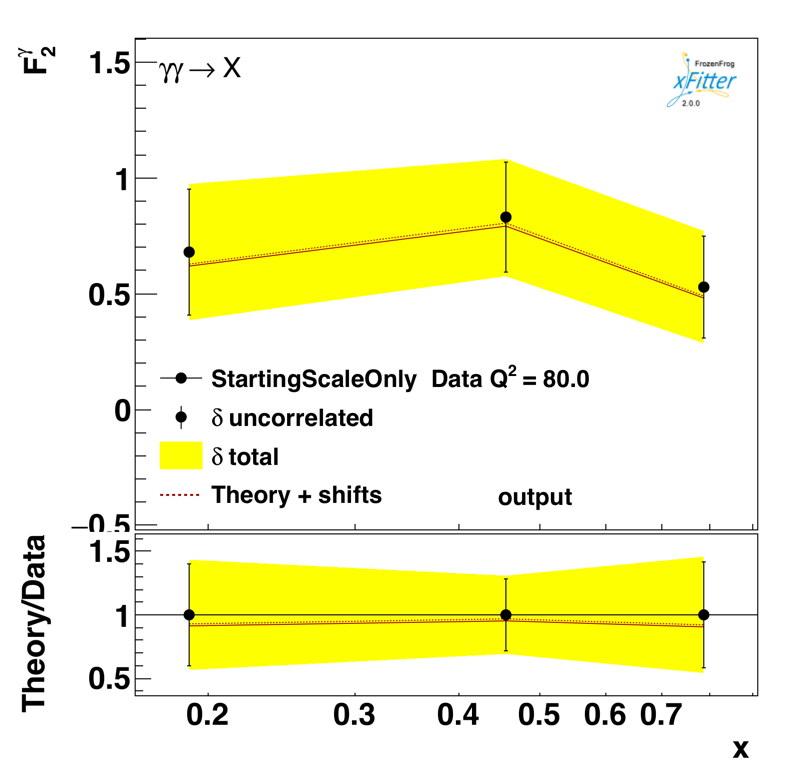
\includegraphics[width=0.4\linewidth]{/Users/schulte/F2_Analysis/10Prozent/Q2_80_0plot.png}
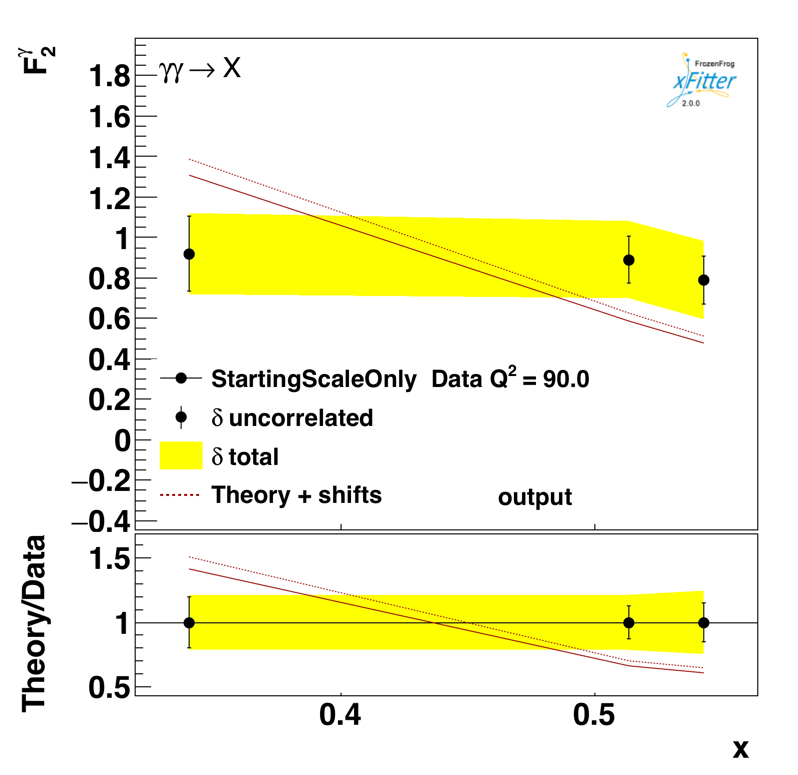
\includegraphics[width=0.4\linewidth]{/Users/schulte/F2_Analysis/10Prozent/Q2_90_0plot.png}\\

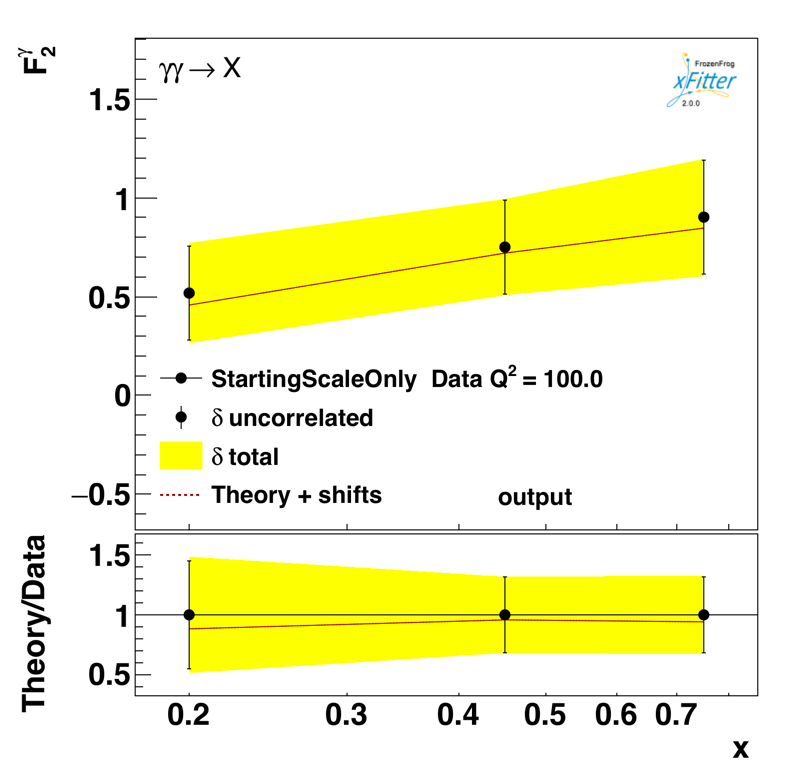
\includegraphics[width=0.4\linewidth]{/Users/schulte/F2_Analysis/10Prozent/Q2_100_0plot.png}
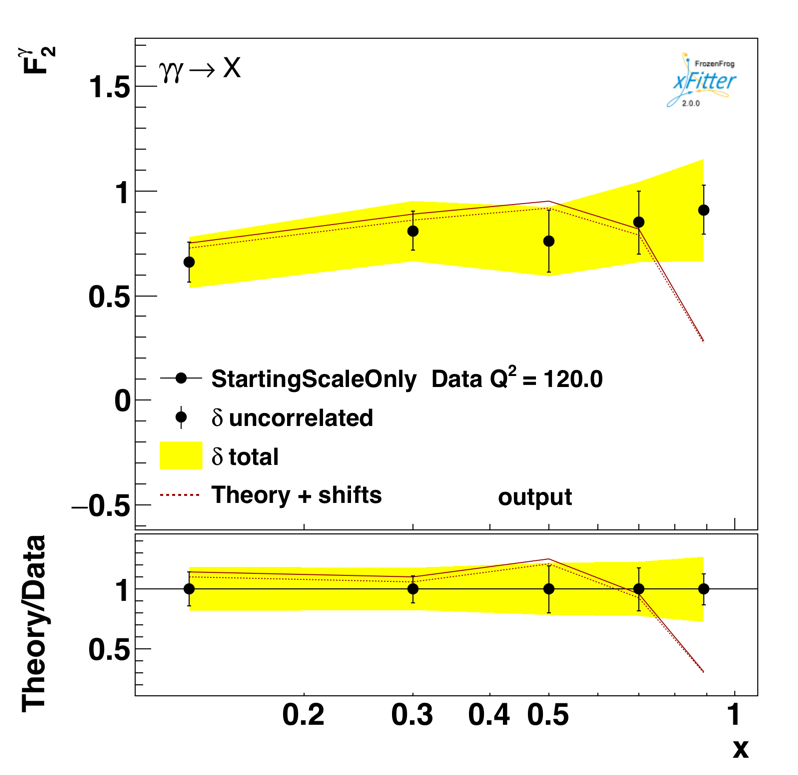
\includegraphics[width=0.4\linewidth]{/Users/schulte/F2_Analysis/10Prozent/Q2_120_0plot.png}\\

\includegraphics[width=0.4\linewidth]{/Users/schulte/F2_Analysis/10Prozent/Q2_125_0plot.png}
\includegraphics[width=0.4\linewidth]{/Users/schulte/F2_Analysis/10Prozent/Q2_135_0plot.png}\\

\includegraphics[width=0.4\linewidth]{/Users/schulte/F2_Analysis/10Prozent/Q2_225_0plot.png}
\includegraphics[width=0.4\linewidth]{/Users/schulte/F2_Analysis/10Prozent/Q2_284_0plot.png}\\

\includegraphics[width=0.4\linewidth]{/Users/schulte/F2_Analysis/10Prozent/Q2_390_0plot.png}
\includegraphics[width=0.4\linewidth]{/Users/schulte/F2_Analysis/10Prozent/Q2_780_0plot.png}

%%%%%%%%%%%%%%%%%%%%%%%%%%%%%%%%%%%%%%%%%%%%%%%%%%



\section*{Acknowledgements}






%%%%%%%%%%%%%%%%%%%%%%%%%%%%%%%%%%%%%%%%%%%%%%%%%
%% REFS %%%
%%%%%%%%%%%%%%%%%%%%%%%%%%%%%%%%%%%%%%%%%%%%%%%%%

\bibliographystyle{JHEP}

\begin{thebibliography}{1}
	%\cite{Acciarri:1998ig}
	\bibitem{Acciarri:1998ig} 
	M.~Acciarri {\it et al.} [L3 Collaboration],
	%``Study of the hadronic photon structure function F(2)**gamma at LEP,''
	Phys.\ Lett.\ B {\bf 436}, 403 (1998).
	doi:10.1016/S0370-2693(98)01025-9
	%%CITATION = doi:10.1016/S0370-2693(98)01025-9;%%
	%78 citations counted in INSPIRE as of 08 May 2018
	
	
	%\cite{Acciarri:1998bh}
	\bibitem{Acciarri:1998bh} 
	M.~Acciarri {\it et al.} [L3 Collaboration],
	%``The Q**2 evolution of the hadronic photon structure function F(2)gamma at LEP,''
	Phys.\ Lett.\ B {\bf 447}, 147 (1999).
	doi:10.1016/S0370-2693(98)01552-4
	%%CITATION = doi:10.1016/S0370-2693(98)01552-4;%%
	%63 citations counted in INSPIRE as of 08 May 2018
	
	
	%\cite{Acciarri:2000rw}
	\bibitem{Acciarri:2000rw} 
	M.~Acciarri {\it et al.} [L3 Collaboration],
	%``Measurement of the photon structure function at high $Q^{2}$ at LEP,''
	Phys.\ Lett.\ B {\bf 483}, 373 (2000)
	doi:10.1016/S0370-2693(00)00587-6
	[hep-ex/0004005].
	%%CITATION = doi:10.1016/S0370-2693(00)00587-6;%%
	%44 citations counted in INSPIRE as of 08 May 2018
	
	
	
	%\cite{Achard:2005fw}
	\bibitem{Achard:2005fw} 
	P.~Achard {\it et al.} [L3 Collaboration],
	%``Measurement of the photon structure function F(2)**gamma with the L3 detector at LEP,''
	Phys.\ Lett.\ B {\bf 622}, 249 (2005)
	doi:10.1016/j.physletb.2005.07.028
	[hep-ex/0507042].
	%%CITATION = doi:10.1016/j.physletb.2005.07.028;%%
	%12 citations counted in INSPIRE as of 08 May 2018
	
	
	%\cite{Akers:1993vw}
	\bibitem{Akers:1993vw} 
	R.~Akers {\it et al.} [OPAL Collaboration],
	%``Measurement of the photon structure function F2 (gamma) in the reaction e+ e- ---> e+ e- + hadrons at LEP,''
	Z.\ Phys.\ C {\bf 61}, 199 (1994).
	doi:10.1007/BF01413097
	%%CITATION = doi:10.1007/BF01413097;%%
	%102 citations counted in INSPIRE as of 08 May 2018
	
	
	%\cite{Ackerstaff:1996se}
	\bibitem{Ackerstaff:1996se} 
	K.~Ackerstaff {\it et al.} [OPAL Collaboration],
	%``Analysis of hadronic final states and the photon structure function F2 (gamma) in deep inelastic electron - photon scattering at LEP,''
	Z.\ Phys.\ C {\bf 74}, 33 (1997).
	doi:10.1007/s002880050368
	%%CITATION = doi:10.1007/s002880050368;%%
	%92 citations counted in INSPIRE as of 08 May 2018
	
	
	%\cite{Ackerstaff:1997ni}
	\bibitem{Ackerstaff:1997ni} 
	K.~Ackerstaff {\it et al.} [OPAL Collaboration],
	%``Measurement of the Q**2 evolution of the photon structure function F2(gamma),''
	Phys.\ Lett.\ B {\bf 411}, 387 (1997)
	doi:10.1016/S0370-2693(97)01023-X
	[hep-ex/9708019].
	%%CITATION = doi:10.1016/S0370-2693(97)01023-X;%%
	%78 citations counted in INSPIRE as of 08 May 2018
	
	
	%\cite{Ackerstaff:1997ng}
	\bibitem{Ackerstaff:1997ng} 
	K.~Ackerstaff {\it et al.} [OPAL Collaboration],
	%``Measurement of the photon structure function F(2)**gamma at low x,''
	Phys.\ Lett.\ B {\bf 412}, 225 (1997)
	doi:10.1016/S0370-2693(97)01022-8
	[hep-ex/9708028].
	%%CITATION = doi:10.1016/S0370-2693(97)01022-8;%%
	%69 citations counted in INSPIRE as of 08 May 2018
	
	
	%\cite{Abbiendi:2000cw}
	\bibitem{Abbiendi:2000cw} 
	G.~Abbiendi {\it et al.} [OPAL Collaboration],
	%``Measurement of the low x behavior of the photon structure function F(2)gamma,''
	Eur.\ Phys.\ J.\ C {\bf 18}, 15 (2000)
	doi:10.1007/s100520000523
	[hep-ex/0007018].
	%%CITATION = doi:10.1007/s100520000523;%%
	%58 citations counted in INSPIRE as of 09 May 2018
	
	%\cite{Barate:1999qy}
	\bibitem{Barate:1999qy} 
	R.~Barate {\it et al.} [ALEPH Collaboration],
	%``Measurement of the hadronic photon structure function at LEP-1 for (Q**2) values between 9.9-GeV**2 and 284-GeV**2,''
	Phys.\ Lett.\ B {\bf 458}, 152 (1999).
	doi:10.1016/S0370-2693(99)00559-6
	%%CITATION = doi:10.1016/S0370-2693(99)00559-6;%%
	%52 citations counted in INSPIRE as of 09 May 2018
	
	
	%\cite{Heister:2003an}
	\bibitem{Heister:2003an} 
	A.~Heister {\it et al.} [ALEPH Collaboration],
	%``Measurement of the hadronic photon structure function F2(gamma)(x, Q**2) in two-photon collisions at LEP,''
	Eur.\ Phys.\ J.\ C {\bf 30}, 145 (2003).
	doi:10.1140/epjc/s2003-01291-4
	%%CITATION = doi:10.1140/epjc/s2003-01291-4;%%
	%13 citations counted in INSPIRE as of 09 May 2018
	
	%\cite{Abreu:1995xta}
	\bibitem{Abreu:1995xta} 
	P.~Abreu {\it et al.} [DELPHI Collaboration],
	%``A Measurement of the photon structure function F2(gamma) at an average Q**2 of 12-GeV**2/c**4,''
	Z.\ Phys.\ C {\bf 69}, 223 (1996).
	doi:10.1007/s002880050022
	%%CITATION = doi:10.1007/s002880050022;%%
	%94 citations counted in INSPIRE as of 09 May 2018
	
	%\cite{Sasaki:1990es}
	\bibitem{Sasaki:1990es} 
	T.~Sasaki {\it et al.} [AMY Collaboration],
	%``A Measurement of the photon structure function $F_2$,''
	Phys.\ Lett.\ B {\bf 252}, 491 (1990).
	doi:10.1016/0370-2693(90)90577-S
	%%CITATION = doi:10.1016/0370-2693(90)90577-S;%%
	%103 citations counted in INSPIRE as of 09 May 2018
	
	%\cite{Sahu:1995gj}
	\bibitem{Sahu:1995gj} 
	S.~K.~Sahu {\it et al.} [AMY Collaboration],
	%``A High Q**2 measurement of the photon structure function F2(gamma),''
	Phys.\ Lett.\ B {\bf 346}, 208 (1995).
	doi:10.1016/0370-2693(95)00092-Y
	%%CITATION = doi:10.1016/0370-2693(95)00092-Y;%%
	%70 citations counted in INSPIRE as of 09 May 2018
	
	
	%\cite{Kojima:1997wg}
	\bibitem{Kojima:1997wg} 
	T.~Kojima {\it et al.} [AMY Collaboration],
	%``A Measurement of the photon structure function F2 (gamma) at Q**2 = 6.8-GeV**2,''
	Phys.\ Lett.\ B {\bf 400}, 395 (1997).
	doi:10.1016/S0370-2693(97)00349-3
	%%CITATION = doi:10.1016/S0370-2693(97)00349-3;%%
	%28 citations counted in INSPIRE as of 09 May 2018
	
	
	%\cite{Muramatsu:1994rq}
	\bibitem{Muramatsu:1994rq} 
	K.~Muramatsu {\it et al.} [TOPAZ Collaboration],
	%``Measurement of the photon structure function F2(gamma) and jet production at TRISTAN,''
	Phys.\ Lett.\ B {\bf 332}, 477 (1994).
	doi:10.1016/0370-2693(94)91284-X
	%%CITATION = doi:10.1016/0370-2693(94)91284-X;%%
	%69 citations counted in INSPIRE as of 09 May 2018
	
	%\cite{Behrend:1983fq}
	\bibitem{Behrend:1983fq} 
	H.~J.~Behrend {\it et al.} [CELLO Collaboration],
	%``Experimental Study of the Hadronic Photon Structure Function,''
	Phys.\ Lett.\  {\bf 126B}, 391 (1983).
	doi:10.1016/0370-2693(83)90187-9
	%%CITATION = doi:10.1016/0370-2693(83)90187-9;%%
	%65 citations counted in INSPIRE as of 09 May 2018
	
	%\cite{Althoff:1986fi}
	\bibitem{Althoff:1986fi} 
	M.~Althoff {\it et al.} [TASSO Collaboration],
	%``Measurement of the Photon Structure Function f(2)Gamma at Q**2 from 7-GeV/c**2 to 70-GeV/c**2,''
	Z.\ Phys.\ C {\bf 31}, 527 (1986).
	doi:10.1007/BF01551073
	%%CITATION = doi:10.1007/BF01551073;%%
	%136 citations counted in INSPIRE as of 09 May 2018
	
	%\cite{Bartel:1982ix}
	\bibitem{Bartel:1982ix} 
	W.~Bartel {\it et al.} [JADE Collaboration],
	%``Experimental Study of the Photon Structure Function F(2) in the High $Q^2$ Region,''
	Phys.\ Lett.\  {\bf 121B}, 203 (1983).
	doi:10.1016/0370-2693(83)90915-2
	%%CITATION = doi:10.1016/0370-2693(83)90915-2;%%
	%48 citations counted in INSPIRE as of 09 May 2018
	
	
	
	%\cite{Aihara:1986xw}
	\bibitem{Aihara:1986xw} 
	H.~Aihara {\it et al.} [TPC/Two Gamma Collaboration],
	%``Measurement of the photon structure function $F_2^\gamma(x,Q^2)$ in the region $0.2< Q^2 < 7$ GeV$^2$,''
	Z.\ Phys.\ C {\bf 34}, 1 (1987).
	doi:10.1007/BF01561108
	%%CITATION = doi:10.1007/BF01561108;%%
	%144 citations counted in INSPIRE as of 09 May 2018
	
	
	%\cite{Aihara:1986xq}
	\bibitem{Aihara:1986xq} 
	H.~Aihara {\it et al.} [TPC/Two Gamma Collaboration],
	%``Observation of scaling of the photon structure function $F_2^\gamma$ at low $Q^2$,''
	Phys.\ Rev.\ Lett.\  {\bf 58}, 97 (1987).
	doi:10.1103/PhysRevLett.58.97
	%%CITATION = doi:10.1103/PhysRevLett.58.97;%%
	%103 citations counted in INSPIRE as of 09 May 2018
	
	%\cite{Abbiendi:2002te}
	\bibitem{Abbiendi:2002te} 
	G.~Abbiendi {\it et al.} [OPAL Collaboration],
	%``Measurement of the hadronic photon structure function F**gamma(2) at LEP-2,''
	Phys.\ Lett.\ B {\bf 533}, 207 (2002)
	doi:10.1016/S0370-2693(02)01560-5
	[hep-ex/0202035].
	%%CITATION = doi:10.1016/S0370-2693(02)01560-5;%%
	%23 citations counted in INSPIRE as of 08 Jun 2018
	
	
	 %\cite{Bartel:1984cg}
	\bibitem{Bartel:1984cg} 
	W.~Bartel {\it et al.} [JADE Collaboration],
	%``Experimental Study of the Photon Structure Function F(2) at Q**2 from 10-GeV**2 to 220-GeV**2,''
	Z.\ Phys.\ C {\bf 24}, 231 (1984).
	%%CITATION = ZEPYA,C24,231;%%
	%152 citations counted in INSPIRE as of 16 Jul 2018
	
\end{thebibliography}




%%%%%%%%%%%%%%%%%%%%%%%%%%%%%%%%%%%%%%%%%%%%%%%%%
\end{document}
%%%%%%%%%%%%%%%%%%%%%%%%%%%%%%%%%%%%%%%%%%%%%%%%%
